%%%%%%%%%%%%%%%%%%%%%%%%%%%%%%
\chapter{Background}

In this chapter, details regarding the simulation theory are gone over.  

%%%%%%%%%%%%%%%%%%%%%%%%%%%%%%
\section{Reactor Analysis}

reactors in general, LWR, fast breeders, GenIV, waste streams, power conversion, coupling between TH, need for fast simulations in oder to do convergence iterations

fission chain reaction, 

\subsection{Seven Factor Formula}
 7 factors

\subsection{Point Kinetics}

\begin{equation}
\label{keff}
k_\mathrm{eff} = 
\end{equation}







%%%%%%%%%%%%%%%%%%%%%%%%%%%%%%
\subsection{History}

The Monte Carlo method is not a new way to simulate nuclear reactors (or any particle transport problem for that matter) and in it's modern form dates back to 1940 when XXX invented the approach while working on the Manhattan Project[cite]. Uncle in Monaco...  During this time, Henry Metropolis and John Von Neumann...[cite]  Although this may be disputed by some people since is was rumored that Enrico Fermi was basically doing small scale simulations of this kind in his head trying to get the Chicago Pile critical [cite].


%%%%%%%%%%%%%%%%%%%%%%%%%%%%%%
\subsection{Nuclear Interactions}
\label{subsec:interactions}

The core of a Monte Carlo simulation is explicitly modeling the individual interactions the neutron undergoes as it moves through matter.  At the highest level, these reactions can be broken down into two categories, elastic reactions and inelastic reactions.  Elastic reactions are those where both momentum and kinetic energy are conserved, i.e. ones where any energy the neutron loses is given to the target nucleus.  Inelastic reactions are those that conserve momentum but do not conserve kinetic energy, i.e. ones where the kinetic energy of the particles can be converted to a vibrational mode of the target nucleus, etc.  These reactions are further divided by the number and type of secondary particles they produce.  Reactions that produce no secondary neutrons are called ``disappearance'' reactions since the neutron effectively disappears, reactions that produce a single neutron are typically called scattering reactions since they effectively change the incoming neutron's energy and direction, and reaction the produce more than one particle are simply called ``secondary-producing'' reactions. Table \ref{nuc_reaction_summary} show a summary of the reaction classifications, and it can be seen that elastic scattering is the only elastic reaction.   

potential scattering vs compound nucleus.

\begin{table}[h]
\centering
\caption{Summary matrix of how neutron reactions are classified.}
\label{nuc_reaction_summary}
\begin{tabular}{| l | c | c | c |}
\multicolumn{4}{c}{Number of Secondaries} \\
\hline
  & 0 & 1 & $>$1 \\
 \hline
 Elastic & & Elastic Scatter & \\
 \hline
 Inelastic & Disappearance & Inelastic Scatter & Secondary-Producing \\
\hline
\end{tabular}
\end{table}

The probabilities for individual reactions occurring are expressed in terms of cross sections.  In simple terms, nuclear cross sections are like a geometric cross sections -they represent the ``size'' of the target nucleus for a particular reaction.  The classical analogy is that if neutrons and nuclei are hard spheres, and neutrons are randomly shot through a material, more neutrons will hit the larger targets than the smaller ones.  Cross sections are also expressed in units of area, the ``barn,'' which is $10^{-24}$ cm$^2$.  This unit was coined by Baker and Holloway while performing scattering experiments with uranium since ``a cross section of $10^{-24}$ cm$^2$ for nuclear purposes was really as big as a barn''\cite{LAMS523}.  Of course, nuclear cross sections have no literal meaning in terms of the actual sizes of the nuclei, they only represent the likelihood of a particular reaction occurring.  Working from the macroscopic scale, which is where measurements are taken, a \emph{macroscopic cross section}, represented by greek capital sigma ($\Sigma$), is the probability of a reaction happening within an infinitesimal distance d$x$.  With this parameter, we can write down an equation that describes the survival probability of a group of particles.  Describing a group is necessary since the dimension x is \emph{continuous}.  Given a particle packet containing N particles and $\Sigma$, their interaction probability over $d$x, the change the population over $d$x is the product of the population N and the interaction probability, as show in \eqref{pop_diff}.

\begin{equation}
\frac{d\mathrm{N}}{d\mathrm{x}} = - \Sigma \mathrm{N}
\label{pop_diff}
\end{equation}

Integrating \ref{pop_diff} over an interval yields an expression for the number of \emph{non-interacting} particles left in a packet after crossing that interval.  Dividing the surviving number by the initial gives a dimensionless expression for the non-interaction probability, P$_\mathrm{NI}$, over the interval x$_1$ as shown in \eqref{pop_NI}.

\begin{equation}
\mathrm{P}_\mathrm{NI} = \frac{\mathrm{N}}{\mathrm{N}_0} = \mathrm{e}^{- \Sigma \mathrm{x}_1}
\label{pop_NI}
\end{equation}

\begin{equation}
\Sigma = \frac{ - \mathrm{ln}(    \mathrm{I} / \mathrm{I}_0  )  }  {\mathrm{x}_1}
\label{pop_beam}
\end{equation}

Since these expressions also apply to beam intensity, they can be used to measure the cross sections for materials by rearranging the equations into the form shown in \eqref{pop_beam}.  If the source intensity, the exiting intensity, and the material thickness are all known, the macroscopic cross section for that material can be determined.  On a microscopic level, however, the neutron interaction probabilities only depend on the type of nucleus, not the aggregate material.  To correct for this, the measured macroscopic cross section can be divided by the number density of nuclei in the material to give the microscopic cross section, $\sigma$, which is material-independent and only depends on the isotope.  In \eqref{micro_exp}, N represents the number density in units of cm$^{-3}$, $\rho$ represents the material density in terms of g*cm$^{-3}$, and M represents the nuclear mass in g.  The microscopic cross section has units of barns, and is what is given in nuclear data files.  They are more general since they are not material-dependent and can be summed into a total material macroscopic cross section by weighting individual microscopic cross sections with the number density of an isotope in a material, as show in \eqref{material_sum_xs}.  In this expression, $f_\mathrm{i}$ is the atomic fraction of isotope i in the material.


\begin{equation}
\Sigma = N \sigma = \frac{\rho}{M} \sigma
\label{micro_exp}
\end{equation}

\begin{equation}
\sum_{\mathrm{i}=1}^{\mathrm{N}_\mathrm{isotopes}} f_\mathrm{i} =1
\label{fraction_norm}
\end{equation}

\begin{equation}
\Sigma_{\mathrm{material}} = \mathrm{N}_1 \sigma_1 +  \mathrm{N}_2 \sigma_2 + \mathrm{N}_3 \sigma_3+ ... = \sum_{\mathrm{i}=1}^{\mathrm{N}_\mathrm{isotopes}} \mathrm{N}_\mathrm{i} \sigma_\mathrm{i} = \rho\frac{\sum_{\mathrm{i}=1}^{\mathrm{N}_\mathrm{isotopes}} f_\mathrm{i}\sigma_\mathrm{i} } { \sum_{\mathrm{i}=1}^{\mathrm{N}_\mathrm{isotopes}} f_\mathrm{i} \mathrm{M}_\mathrm{i}}
\label{material_sum_xs}
\end{equation}

The above expressions do not take energy into account, so they are assumed to be at a single energy.  Using such simple expressions to determine the cross section of an isotope would only be valid with the use of a very, very precisely mono-energetic beam.  The quantum mechanical details that go into cross sections can cause them to depend strongly on the energy (or velocity) of the neutron and the target nucleus.  Many nuclides have resonances where the interactions probability spikes to very large values.  This typically happens when the incoming energy is exactly that of an energy level of the resultant compound nucleus \cite{duderstadt}.   Figure \ref{xs_e_dependence_li} shows the energy dependence of various reactions type in lithium-6 and Figure \ref{xs_e_dependence_u} shows the dependence of others in uranium-235.  

\begin{figure}[h!]
  \centering
    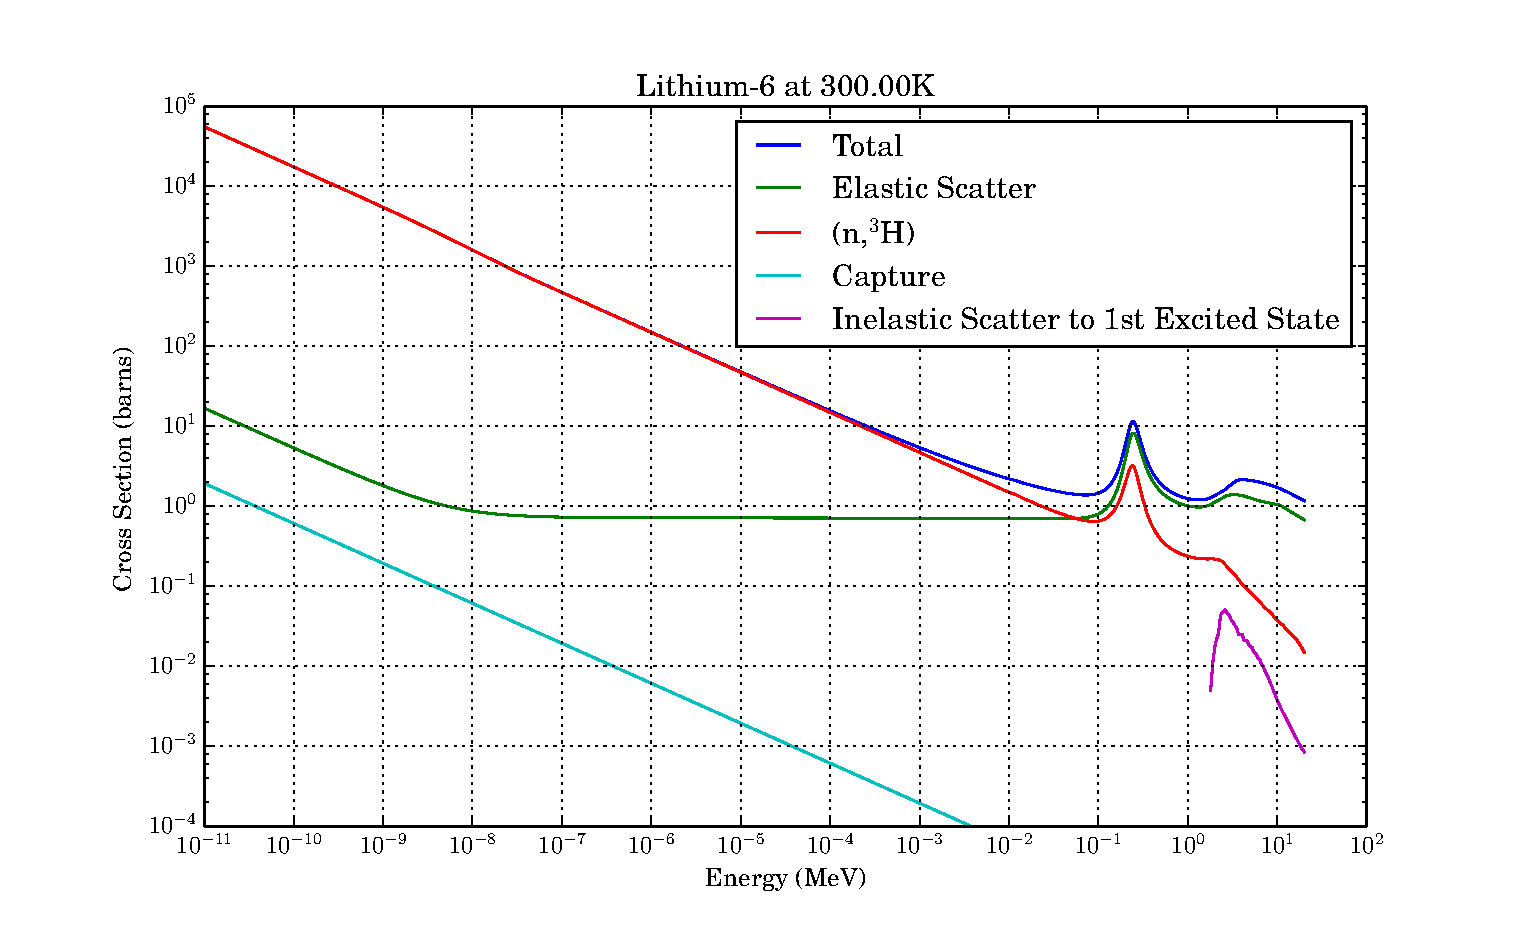
\includegraphics[width=0.8\textwidth]{graphics/xs_li6.eps}
     \caption{The energy dependence of some reactions in lithium-6.\label{xs_e_dependence_li}}
\end{figure}

\begin{figure}[h!]
  \centering
    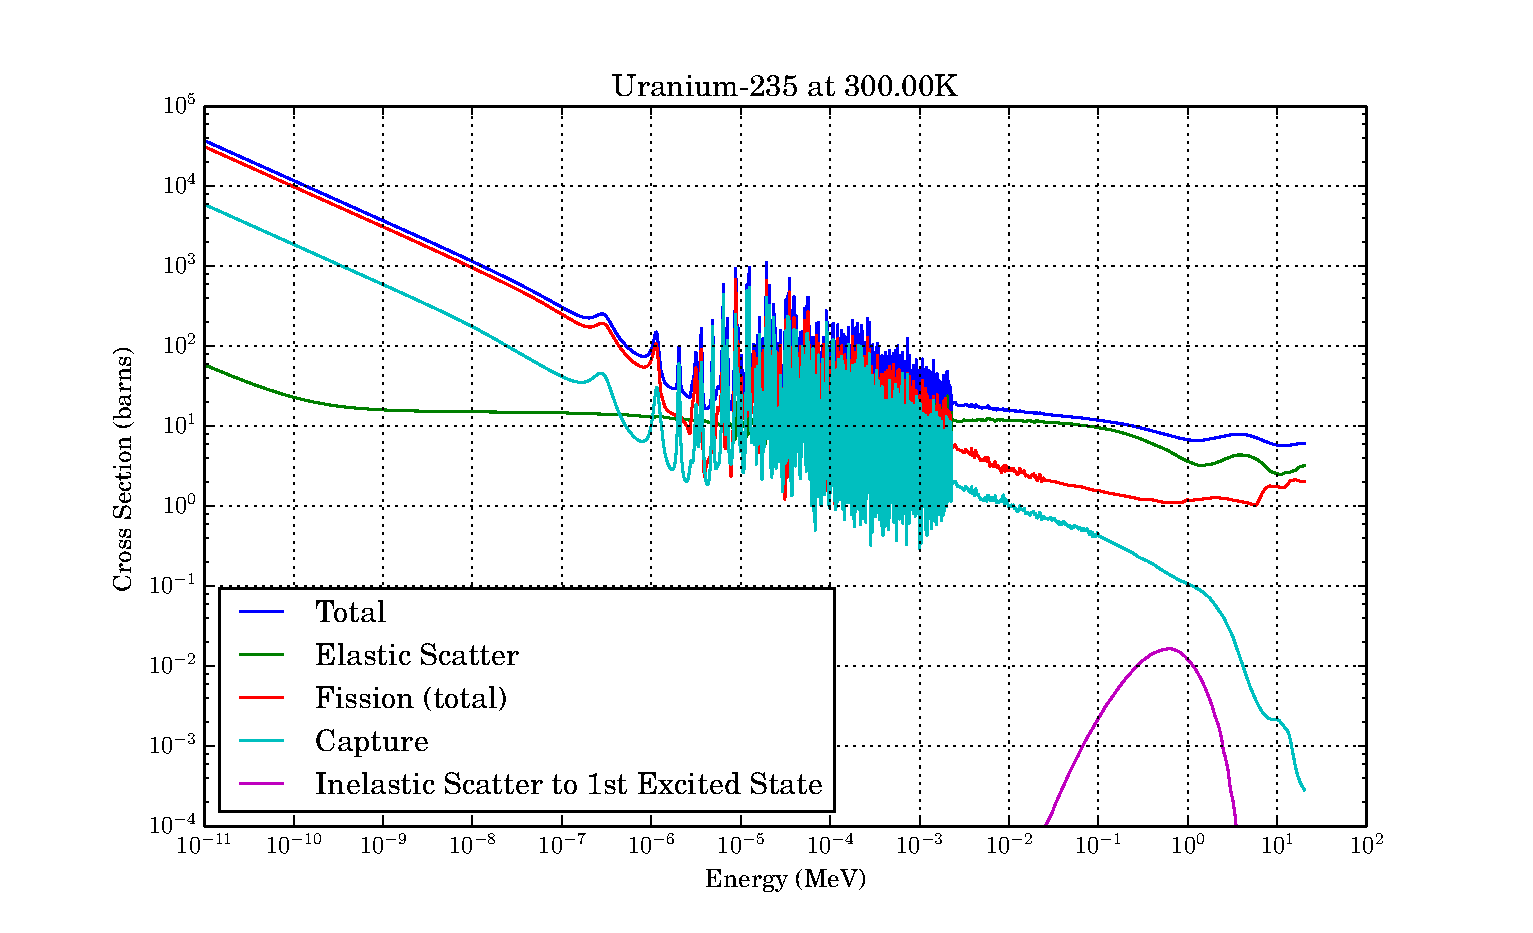
\includegraphics[width=0.8\textwidth]{graphics/xs_u235.eps}
    \caption{The energy dependence of some reactions in uranium-235.   \label{xs_e_dependence_u}}
\end{figure}

It is important to note the complexity shown in uranium-235 in the 0.1eV to 40keV range.  This is referred to as the ``resonance region'' and adds much of the complexity in accurately modeling neutron transport.  There are no simple functional representations available for these types of cross sections, so they must be represented in a point-wise tabular format.  It is also important to note that at low energies, cross sections typically lose structure and exhibit the same ``1/$v$'' scaling.  This is due to the particle and the target having more time to interact with each other.  The energy levels where this phenomenon exists is similar the thermal energy of the target and the target no longer appears stationary from the neutrons perspective.  If the neutron is slow enough, the targets appear to be moving instead of the neutron, and more of them come into the neutrons sphere of interaction.  This is the qualitative reason for 1/$v$ scaling at low energies.  Due to to their identical scaling, the ratios between the reaction types stays constant as velocity is decreased but the overall interaction probability with respect to distance increases.

In the next subsections, the characteristics and kinematics of the different reaction types are explained.

\subsubsection{Elastic Scattering}

Elastic scattering conserves both the momentum and the kinetic energy of the reacting particles and occurs when the neutron does not enter the nucleus, only bounces off of it's potential field.  Since there is only a single exiting particle, elastic scattering is a two-body interaction and the exiting energies can be determined if the angle between the exiting particle is known.  This problem is greatly simplified if the interacting particles' velocities are transformed into the center-of-mass (CM) frame, where net momentum is zero. The velocity of the CM is defined in \eqref{vCM} where $m$ and $M$ are the neutron's and the target's respective masses, $v$ and $V$ are their respective velocity vectors, and $A$ is the ratio of the target's mass to the neutron's mass (also know as the ``atomic weight ratio'' or AWR).  The derivation from here follows closely with that in ref \cite{jaakko}.

\begin{equation}
A = \frac{M}{m}
\label{AWR}
\end{equation}

\begin{equation}
\boldsymbol{v_{\mathrm{CM}}} = \frac{ m \boldsymbol{v} + M \boldsymbol{V} }    {m+M} = \frac{ \boldsymbol{v} + A \boldsymbol{V} }    {1+A}
\label{vCM}
\end{equation}

The CM velocities of the target and the neutron are then calculated by subtracting the CM velocity out of them, ash shown in \eqref{CM}.  The $_\mathrm{c}$ subscript will denote the CM-frame values from now on, whereas $v_{\mathrm{CM}}$ will denote the velocity of the CM frame relative to the lab frame.

\begin{equation}
\begin{split}
 \boldsymbol{v_{_\mathrm{c}}} &= \boldsymbol{v} - \boldsymbol{v_{\mathrm{CM}}} \\  
 \boldsymbol{V_{\mathrm{c}}} &= \boldsymbol{V} - \boldsymbol{v_{\mathrm{CM}}}
 \end{split}
\label{CM}
\end{equation}

Once in the CM frame, the equation for conservation of momentum can be written as \eqref{consMomCM}.  The primed values are those after the collision.  Since the net momentum is zero, the directions of the neutron and the target must be in opposite directions as shown in \eqref{rotationCM}.

\begin{equation}
\begin{split}
m \boldsymbol{v_{_\mathrm{c}}} + M \boldsymbol{V_{_\mathrm{c}}} &= m \boldsymbol{v_{_\mathrm{c}}^\prime} + M \boldsymbol{V_{_\mathrm{c}}^\prime} = 0\\
    \boldsymbol{v_{_\mathrm{c}}} + A  \boldsymbol{V_{_\mathrm{c}}} &=     \boldsymbol{v_{_\mathrm{c}}^\prime} + A  \boldsymbol{V_{_\mathrm{c}}^\prime} = 0
\end{split}
\label{consMomCM}
\end{equation}

\begin{equation}
\begin{split}
\boldsymbol{v_{_\mathrm{c}}^\prime} &= - A  \boldsymbol{V_{_\mathrm{c}}^\prime} \\
\boldsymbol{v_{_\mathrm{c}}} &= -A  \boldsymbol{V_{_\mathrm{c}}}
\end{split}
\label{rotationCM}
\end{equation}

The equation for conservation of energy is shown in \ref{consECM}.  Energy is a scalar quantity, and therefore these equations are as well.  There are no vectors, which are indicated with boldface type, since $v^2 =( \boldsymbol{v} \cdot \boldsymbol{v})$.  $Q$ is the amount of energy released by the reaction, and is zero here but is convenient to include in this derivation for use in inelastic collision kinematics where it is nonzero.

\begin{equation}
\begin{split}
m v_{_\mathrm{c}}^2 + M V_{_\mathrm{c}}^2 &= m v_{_\mathrm{c}}^{\prime2} + M V_{_\mathrm{c}}^{\prime2} + 2Q \\
    v_{_\mathrm{c}}^2 + A  V_{_\mathrm{c}}^2 &=     v_{_\mathrm{c}}^{\prime2} + A  V_{_\mathrm{c}}^{\prime2} + \frac{2Q}{m}
\end{split}
\label{consECM}
\end{equation}

There are now two unknowns (the primed values) and two equations, and the final velocities of the neutron and the target can be determined.  Substituting \eqref{rotationCM} into \eqref{consECM} and solving yields either equation in \eqref{finalvCM}, depending on how the substitution is done.  It can be seen that if $Q$ is zero, as it is in elastic scattering, the initial and final velocities are the same for the particles and the interaction only causes a rotation in the CM frame.

\begin{equation}
\begin{split}
v_{_\mathrm{c}}^{\prime} &=  \sqrt{ v_{_\mathrm{c}}^{2} + \frac{2AQ}{m(A+1)}  }  \\
V_{_\mathrm{c}}^{\prime} &= \sqrt{ V_{_\mathrm{c}}^{2} + \frac{2Q}{mA(A+1)}  } 
\end{split}
\label{finalvCM}
\end{equation}

At first glance, it seems like the interaction has been fully characterized, but \eqref{rotationCM} only relates the initial states of the neutron and the target to one another and the final states of neutron and the target to one another.  The initial state and final state of the neutron still need to be related.  It has been mentioned already that the interaction is only a rotation in the CM frame, so the initial and final state of the neutron's direction can be related by a three-dimensional rotation formula.  An efficient algorithm is given by the Rodrigues' rotation formula, shown in \eqref{RodriguesRot}.  In the formula, $\boldsymbol{k}$ is an auxilliary unit vector around which $\boldsymbol{v}$ is being rotated.  From this unit vector, $theta$ is the angle $\boldsymbol{v}$ is rotated away from $\boldsymbol{k}$ such that $(\boldsymbol{v} \cdot \boldsymbol{v_{\mathrm{rot}}}) = |v||v_{\mathrm{rot}}|\cos\theta$.  It is ``efficient'' in the sense that to rotate a vector, a full 3x3 matrix does not need to be constructed and multiplied by the vector. In other words, matrix-vector operations are not needed and it can be carried out with only vector operations \cite{}.

\begin{equation}
 \boldsymbol{ v_{ \mathrm{rot}}} = \boldsymbol{v} \cos \theta + (\boldsymbol{k} \times \boldsymbol{v}) \sin \theta + \boldsymbol{k} (\boldsymbol{k} \cdot \boldsymbol{v})(1-\cos \theta)
\label{RodriguesRot}
\end{equation}

If the polar and azimuthal rotation angles, $\theta$ and $\phi$, respectively, are determined, the initial neutron velocity vector can be rotated through these angles to its final value.  After the rotation is done, the final velocities are known in the CM frame and they can be transformed back to the lab frame to give the final velocities there, as shown in \eqref{xformbackCM}.

\begin{equation}
\begin{split}
 \boldsymbol{v^{\prime}}  &= \boldsymbol{v_{\mathrm{c}}^{\prime}} + \boldsymbol{v_{\mathrm{CM}}} \\  
 \boldsymbol{V^{\prime}} &= \boldsymbol{V_{\mathrm{c}}^{\prime}} + \boldsymbol{v_{\mathrm{CM}}}
 \end{split}
\label{xformbackCM}
\end{equation}


\subsubsection{Inelastic Level Scattering}

Inelastic scattering is the other type of scattering a neutron can undergo where kinetic energy is no longer conserved.  An amount of energy is either released from the reaction to the particles, or more commonly, taken from the particles and lost to the reaction.  In neutron-nucleus collisions, the target nucleus can be excited to a higher energy state than its ground state if the colliding neutron has a high enough energy to do so.  If it does and the collision excites the nucleus, a discrete amount of energy equal to the energy of the excited state is lost to the reaction.  These excited states typically do not have long half lives, and a gamma ray is emitted when the nucleus relaxes to its ground state.  This type of reaction is called inelastic level scattering due to a an excited energy \emph{level} becoming occupied by the target nucleus.  

Since it is still a two-body interaction, the kinematics of the reaction are identical to elastic scattering except the $Q$ value is nonzero and negative.  These reactions have a threshold energy below which their cross sections are zero since the neutron would not have enough energy to excite the state.   Figure \ref{Elevels} shows the energy levels in lead-XXX, which is often used as a fast neutron moderators due to its many, low-lying energy levels and its large inelastic scattering cross sections.

\begin{figure}[h!]
  \centering
    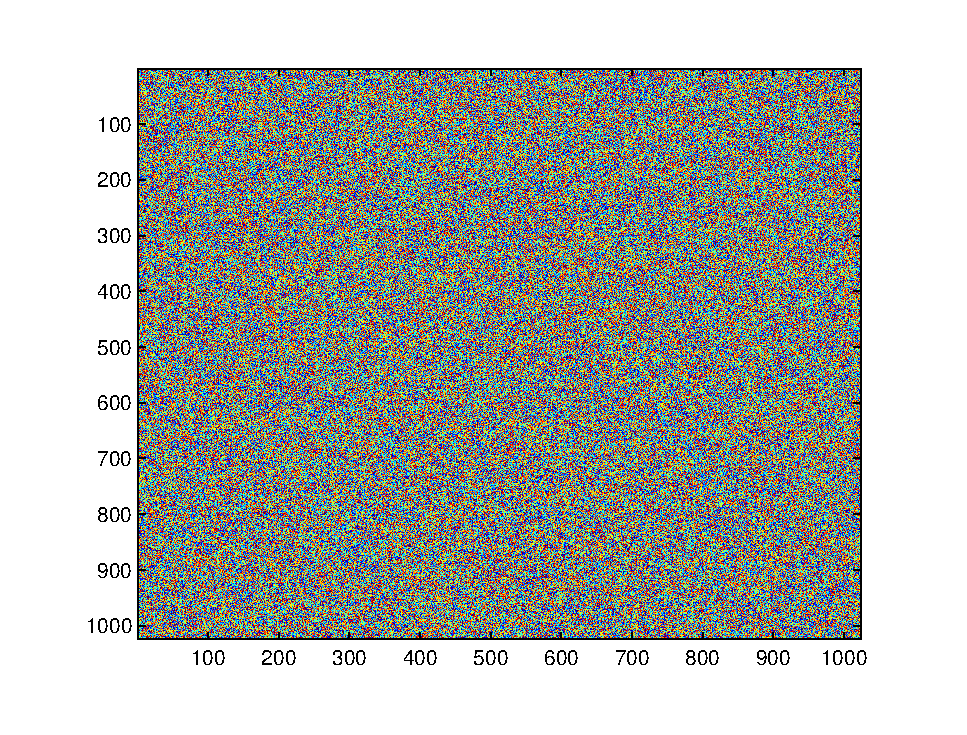
\includegraphics[width=0.8\textwidth]{graphics/noise.eps}
     \caption{The energy levels of lead-XXX\cite{}. \label{Elevels}}
\end{figure}

\subsubsection{Inelastic Continuum Scattering}

At energies above the distinct levels there lies a continuum in the nuclear energy states.  This isn't truly a ``continuum'' in the strictest sense, but the energy levels become so close together they they effectively form a domain where energy can take continuous values.  Unlike the discrete $Q$ values corresponding to a single excited state used in inelastic level scattering, the $Q$ value of the reaction now follows a distribution.  

In bound nuclei, S(a,b)

\subsubsection{Disappearance Reactions}

Unlike scattering reactions, where the energy and direction of the neutron is changed but continues to transport, \emph{disappearance} reactions remove a free neutron.  Typically this \emph{capture} of a neutron leaves the daughter nucleus in an excited state, which them relaxes to ground state by emitting a gamma ray.


\subsubsection{Fission}

Fission means ``the splitting splitting of something into two parts'' in the literal sense of the word.  This is exactly what nuclear fission is as well.  It is when a nucleus splits into two smaller nuclei, called \emph{fission fragments}.  When heavy nuclei undergo fission, they release energy, and typically emit a few other particles, including neutrons.  That this reaction releases energy is the reason heavy elements, like uranium, can be used as an energy source.  This is because the fission fragments have a higher binding energy per nucleon compared to the parent nucleus.  Figure \ref{binding_e_per_nuc} shows the average binding energy per nucleon for a wide range of isotopes.  Note that the peak of the curve is at Iron-56, the most tightly bound nucleus, and that heavier nuclides are lower than it.  Fission splits the parent into two lighter nuclides, and since the fragments are more tightly bound, the excess binding energy from the parent is released.  The released energy isn't simply deposited as heat directly, however, it is released in a range of forms.  Fission doesn't just release some energy, it releases a substantial amount of it.  Uranium-235, for example, releases a total of 192.9$\pm$0.5 \emph{MeV} per fission \cite{duderstadt}.  Compared to chemical energy sources where the energy released per reaction is on the order of 1\emph{eV}.  Fission energy yield is 8 orders of magnitude larger!  Not all of this energy is converted to heat, bit a substantial amount is.  Table \ref{fission_dist} shows the fraction of this total energy that is given to each entity.  Note that a significant fraction is given to neutrinos, which is essentially lost due to their very small interaction cross section.  The kinetic energy of the fission fragments has the majority of the energy, and since they are heavy and charged, their energy is deposited as heat very near to the fission site.  Other particles, light photons and neutrons, carry some of the fission energy further away from the fission site, but their energy mostly still ends up as heat.
  
\begin{figure}[h!]
  \centering
    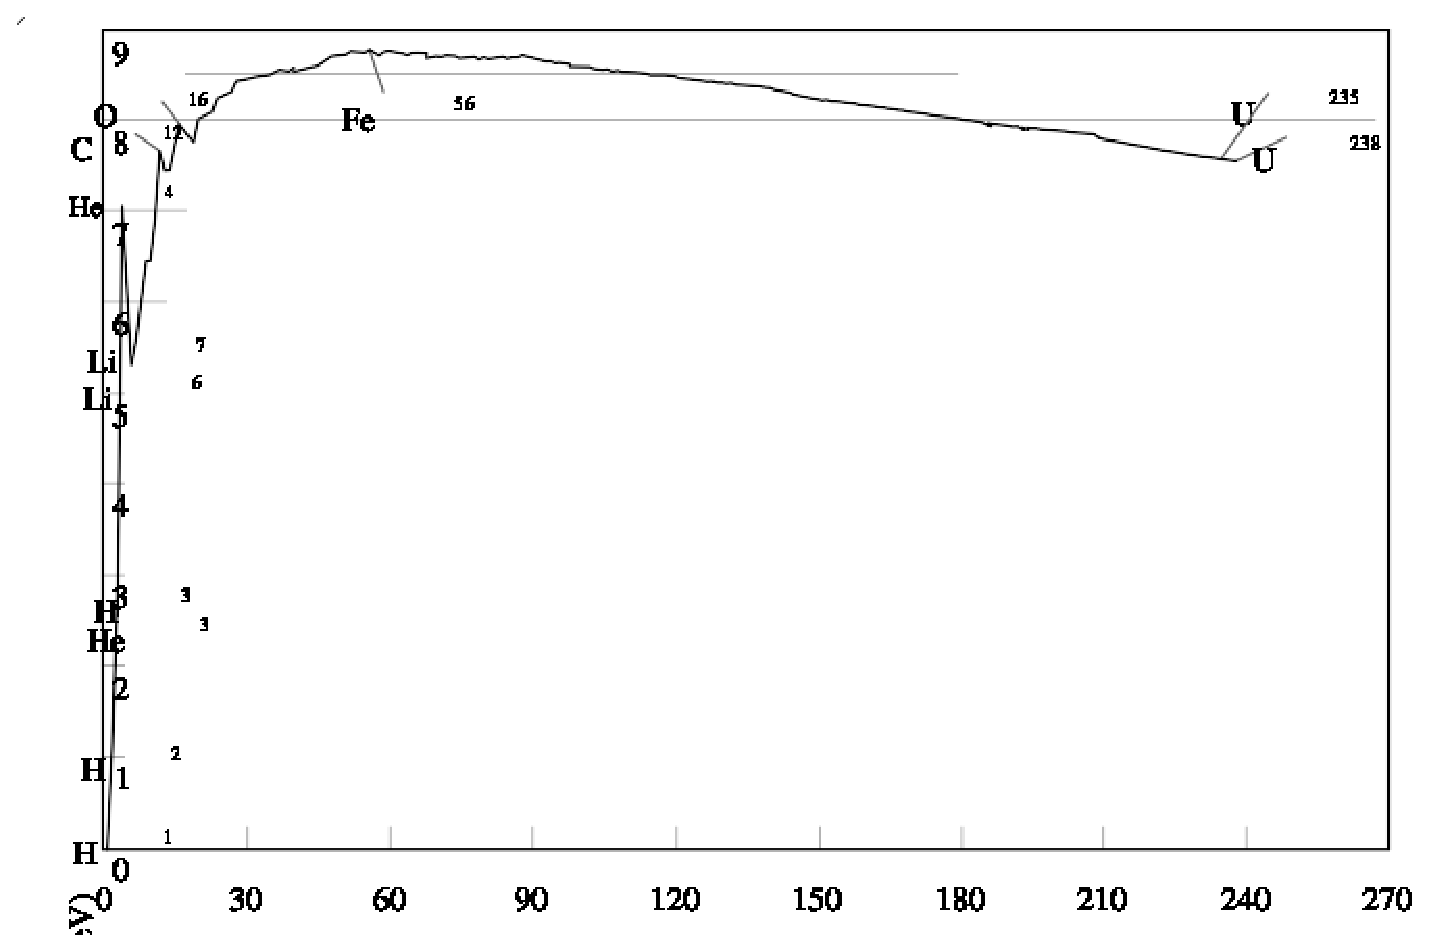
\includegraphics[width=0.8\textwidth]{graphics/binding_e_per_nuc.eps}
     \caption{Average binding energy per nucleon.  REPLACE ME WITH ONE YOU MAKE YOURSELF FROM DATA. \cite{}.\label{binding_e_per_nuc}}
\end{figure}

\begin{table}[h]
\centering
\caption{Average distribution of fission energy \cite{duderstadt}.\label{fission_dist}}
\begin{tabular}{| l | c | r | r |}
\hline
Particle & Energy (\%) & Range & Time \\
\hline
Fission fragment kinetic energy & 80 & $<$0.1cm & prompt \\
\hline
Prompt neutrons & 3 & 10-100cm & prompt \\
\hline
Photons & 4 & 100cm & prompt \\
\hline
Fission product $\beta$ decay & 4 & short & delayed \\
\hline
Neutrinos &  5 & extremely long & delayed \\
\hline
Nonfission reactions from n capture & 4 & 100cm & delayed \\
\hline
\end{tabular}
\end{table}

Fission is technically considered a disappearance reaction as well since the fission-inducing neutron is absorbed by the nuclide.  Even though is is absorbed, more than 2 new neutrons are released by fission, enabling the fission chain reaction to occur.  An important parameter of the fission chain reaction is $nu$, the fission neutron yield.    The total yield is different than the prompt yield in that it also includes neutrons produced from photon-induced emission and from fission product decay.  These neutrons are not ``prompt'' in that they are not emitted immediately from the fission itself.  The processes that create these ``delayed'' neutrons (decay and nuclear relaxation) take time to occur.  Prompt neutrons appear immediately after fission, whereas delayed neutrons can appear anywhere between 0.6 to 80 seconds after.  The kinetics of a nuclear chain reaction depend heavily on the fraction the delayed neutrons which sustain the chain reaction.  Since they have a relatively large time delay, they cause the time between subsequent neutron generations to become longer.  This time between generations is called the \emph{effective neutron lifetime}, and is approximately $10^{-4}$ seconds for prompt neutrons and $0.1$ seconds for delayed neutrons in light water (thermal spectrum) reactors \cite{duderstadt}.  

\begin{figure}[h!]
  \centering
    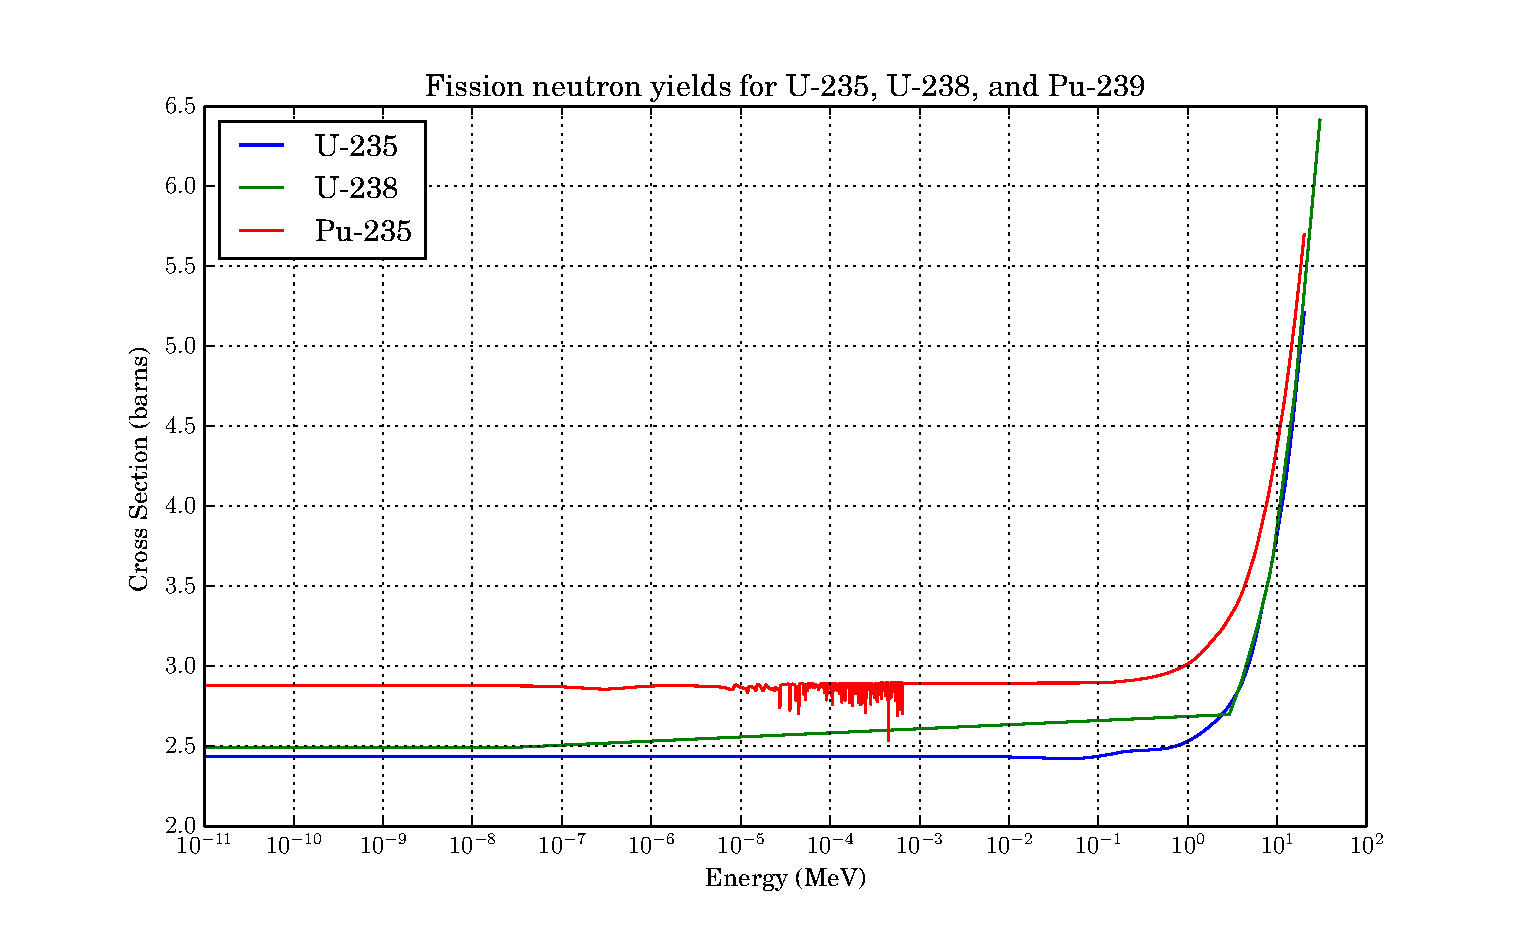
\includegraphics[width=0.8\textwidth]{graphics/nu_compare.eps}
     \caption{Total fission yield, $\nu_\mathrm{T}$, for uranium-235, uranium-238, and plutonium-239. \label{nu_compare}}
\end{figure}

\begin{figure}[h!]
  \centering
    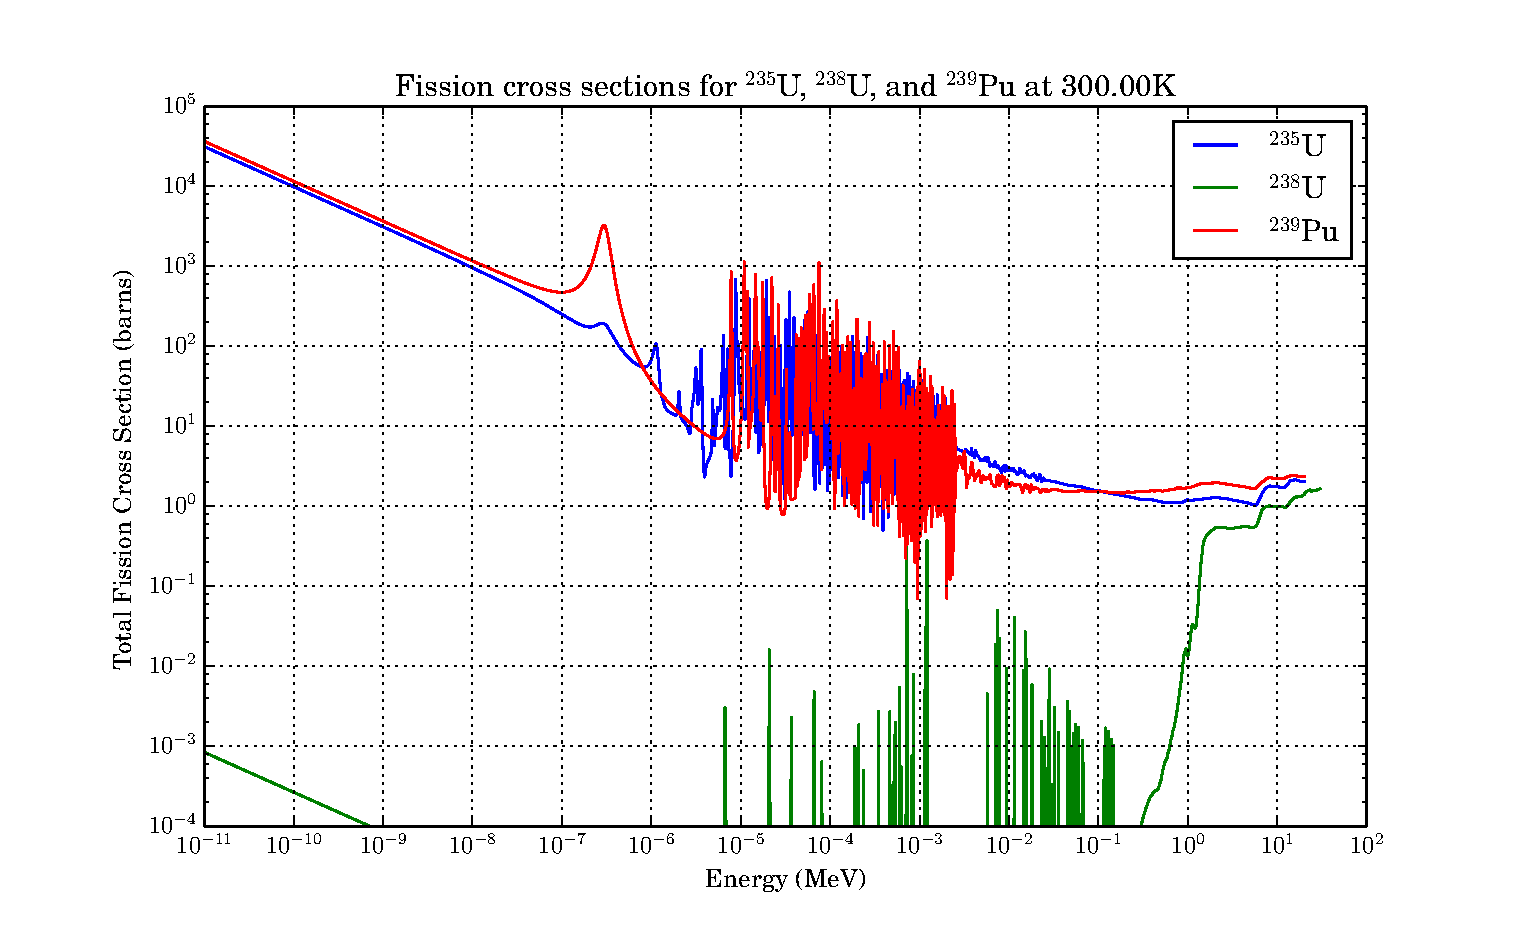
\includegraphics[width=0.8\textwidth]{graphics/xs_fissile.eps}
     \caption{Fission cross sections for uranium-235, uranium-238, and plutonium-239. \label{xs_fission_only}}
\end{figure}

Figure \ref{nu_compare} shows the energy dependence of the total fission neutron yield, $nu_\mathrm{T}$. It is shown at one temperature since it have very weak temperature dependence.   It can be seen that it is constant until energies in the MeV range, where it increases sharply due to the energy the incident neutron provides being sufficient to eject a bound neutron.  Figure \ref{xs_fission_only} shows the total fission cross sections for two \emph{fissile} isotopes, uranium-235 and plutonium-239, and one \emph{fertile} isotope, uranium-238.  Fissile isotopes are those which neutrons at any energy can induce fission.  The figure shows that uranium-238 has a fission cross section, but it isn't significant until above 1 MeV.  For uranium-238, fission is a threshold reaction.  Simply absorbing a neutron does not provide enough energy to split the nucleus.  Additional energy is required, which can be provided in the form of an incident neutron's kinetic energy.  Uranium-238 isn't fissile, but it can be a significant contributor of fission reactions in reactors where the neutron population is \emph{fast}, i.e. mainly high-energy.  As mentioned before, uranium-238 is considered fertile, which means that it produces a fissile isotope after it absorbs a neutron, and in this case decays to plutonium-239.  

Fission spectrum?

\subsubsection{Other Inelastic Secondary-Producing Reactions}

This category encompasses all the other reactions neutrons undergo.  There are two types, ones that produce secondary neutrons in some amount and those that do not.  Those that do not may still produce other particles, like alpha particles, tritons, protons, et cetera.  Since they do not produce secondary neutrons, however, they are basically equivalent to a disappearance reaction in the scope of neutron transport.  Even though they aren't capture reactions, they can contribute significantly to an isotope's absorption of neutrons.  Figure \ref{xs_e_dependence_li} shows that the (n,$^3$H) in lithium-6 is by far the main component of the total cross section and makes it a very strong absorber of low energy neutrons.  Boron-10 is another great example of this.  Its (n,$\alpha$) reaction has a very high cross section for low energy neutrons, and it is widely used in thermal spectrum reactors in safety and control systems.

Of the reactions that produce secondary neutrons, the (n,2n) reaction is most significant, due to it having the lowest threshold energy.  At higher incident neutron energies, (n,3n) and even (n,4n) can become possible.  Other particle combinations are possible as well, such as (n,n$\alpha$), and these reactions act like an inelastic scatter interaction where the relationship between scattering angle and energy no longer applies due to there being three bodies to distribute energy to instead of only two.

%%%%%%%%%%%%%%%%%%%%%%%%%%%%%%
\subsection{Temperature Effects}
\label{sec:temp}

Thus, far there has only been mention of the target nuclide's by how it manifests itself in the 1/$v$ behavior of cross sections at low energy.  Most of the time, it is a good assumption that the thermal motion of the target nuclide is negligible.  Thermal energy is on the order of .01 eV, and this is a good assumption when neutrons are at MeV range energies, but when they scatter and lose energy, they can come near the thermal energy of the material.  When this happens, the target nuclide no longer appears stationary, and assuming that it has zero velocity in scattering calculations is inaccurate.  MCNP sets the threshold at 400kT, which corresponds to about 10 eV for materials at room temperature, above which the target nuclide can be assumed stationary.  Below this threshold, it is important to model thermal effects.  If this wasn't done, a neutron could keep scattering off of zero-energy targets and it's energy could approach zero, which is not physical.  Neutrons can only scatter down to a state where they are in thermal equilibrium with the material they are traveling through.  This creates a ``thermal peak'' at low energies where neutrons collect, especially in materials where the scattering cross section is large and neutrons scatter many times before they are absorbed.

\begin{figure}[h!]
  \label{MB_dist}
  \centering
    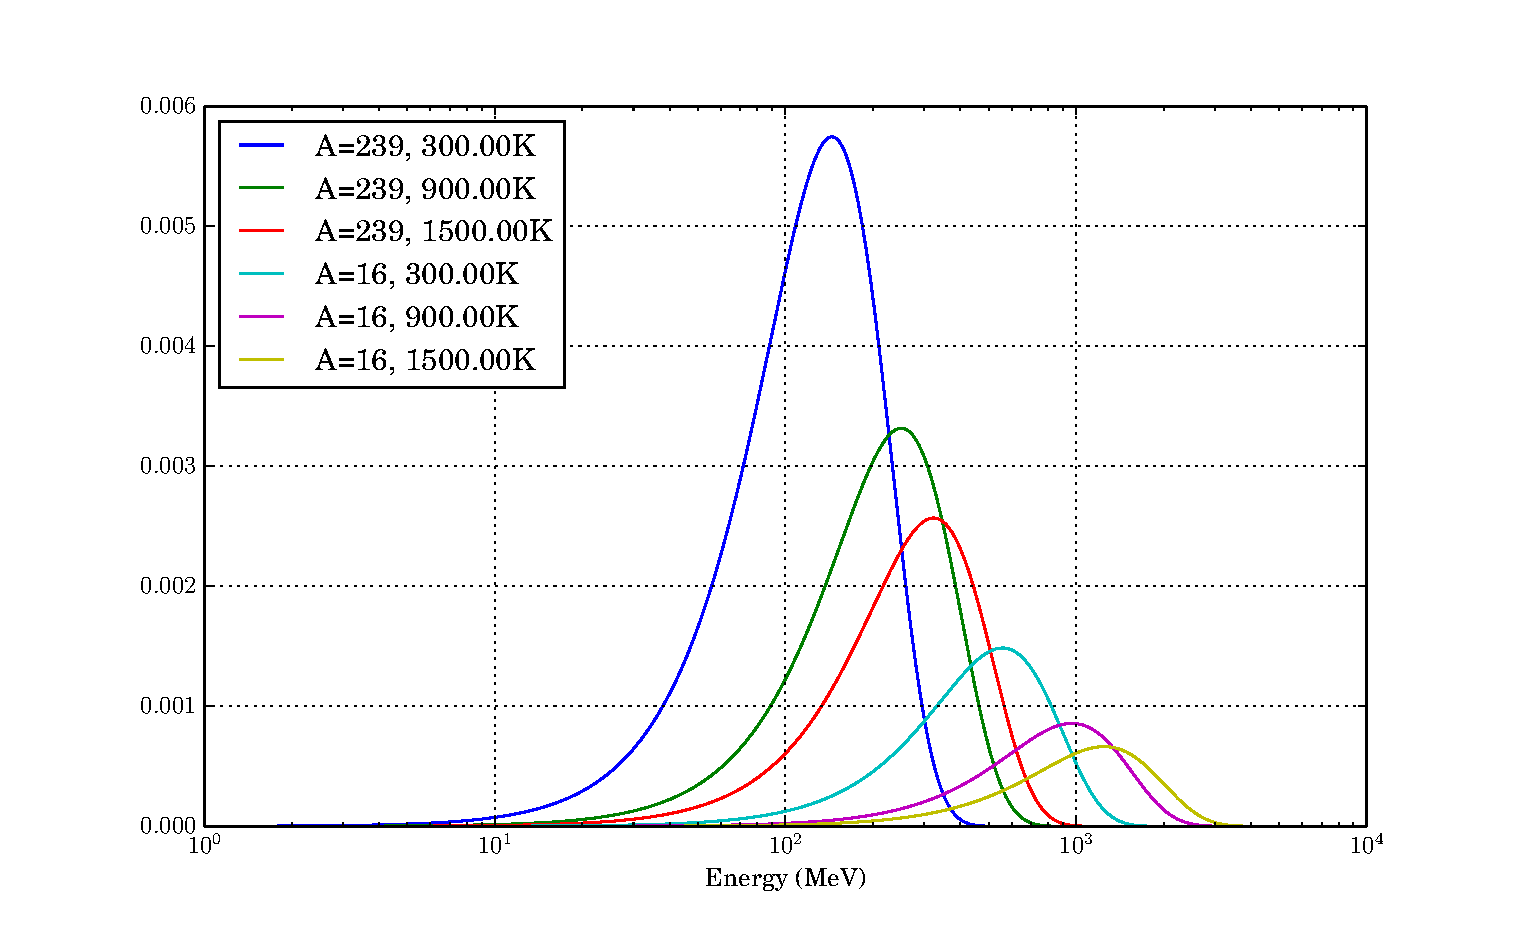
\includegraphics[width=0.8\textwidth]{graphics/MB_dist.eps}
     \caption{Maxwell-Boltzmann distribution for the speed of heavy and light nuclides at different temperatures.}
\end{figure}


\subsubsection{Doppler Effect}


The other effect that thermal motion has is the \emph{Doppler effect}.  This is where resonances are broadened as temperature increases due to the thermal distribution becoming wider.  The effect is also known as \emph{Doppler broadening} for this reason.  Figure \ref{MB_dist} shows the Maxwell-Boltzmann distributions at various temperatures for a heavy particle and for a light particle.  This is the distribution of speeds particles in a ``gas'' have if they only interact by scattering off of one another.  Most solids can be modeled as a dense gas when there are no strong anisotropies in their structure, which is why modeling the target velocities in this way is called the ``free gas model.''  Note that the broadening effect is much more pronounced for light nuclei.  

The widening of resonances effects reactors in significant ways, most notably in that more neutrons are absorbed in the resonance region as the scatter down to thermal energies.  The number of neutrons lost to capture increases and reduces the overall multiplication factor.  It is important for reactor safety that this occurs since it produces a negative reactivity feedback for temperature and helps prevent power excursions and meltdowns.  If the multiplication factor is above unity, the power starts to rise, and therefore so does the temperature (if the coolant flow rate remains the same).  When the temperature goes up, the increased captures causes it to go back down, stopping the power from increasing.  Of course, there are many different types of reactivity feedback phenomena, but the temperature feedback is generally negative due to Doppler broadening.  Capture is increases most in fission products since they often have strong absorption resonances and are lighter than fuel nuclides.  Very light nuclides typically do not have absorption resonances, so Doppler broadening has littler effect on their absorption rates.  This is why temperature feedback is least effective in fresh fuel where there are few fission products.  Figure \ref{xs_eu_broaden} shows the effect in europium-155, a fission product with a high capture cross section.

\begin{figure}[h!]
  \centering
    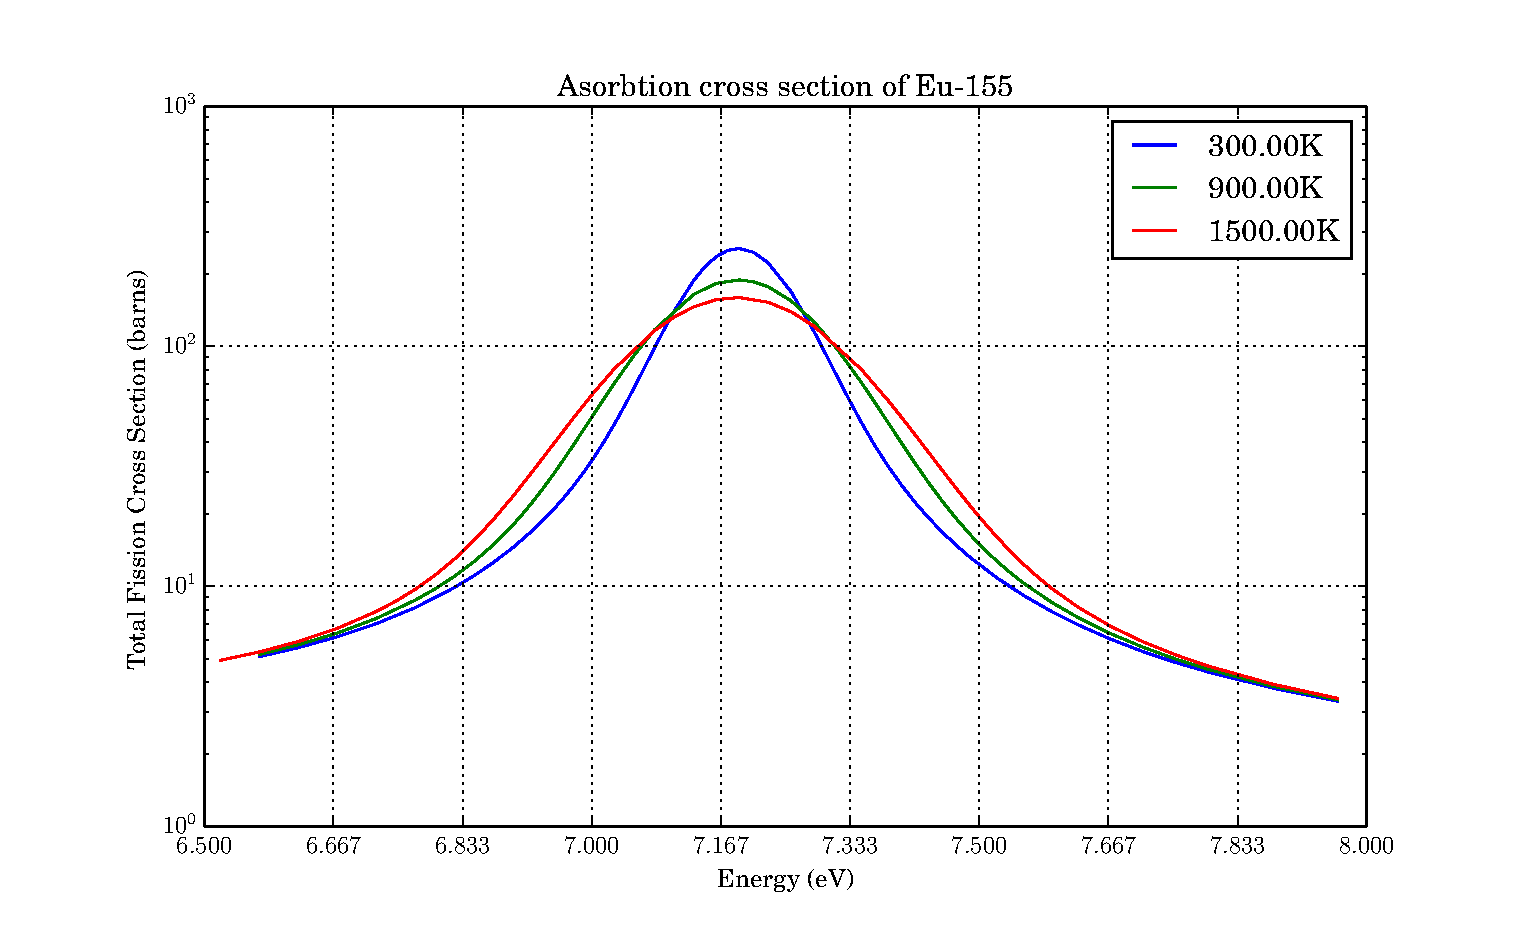
\includegraphics[width=0.8\textwidth]{graphics/xs_eu_broaden.eps}
     \caption{Doppler broadening of the 1eV fission resonance in Eu-155.  \label{xs_eu_broaden}}
\end{figure}

At 0K, resonances are very sharp and can be treated as delta functions.  The reaction rates actually depend on the relative velocity of the neutron and the target nuclide, and since the target nuclides have a spectrum of energies, the relative velocity does as well.  Assuming the target is at rest requires summing all the contributions to the reaction rate from the different relative velocities given a single neutron energy.  From the reaction rate, a \emph{thermally averaged} cross section can be calculated be used in simulations assuming a target at rest.  This is especially significant at resonances since slight movements in velocity can produce very large differences in cross section.  The overall effect is that sharp resonances are \emph{effectively} broadened since they start to contribute to reaction rates once the thermal distribution of relative velocities starts overlap them.   The expression for thermally averaged cross section is shown in \eqref{broaden}, where $v_n$ and $\boldsymbol{v_n}$ are the velocity and speed of the neutron, respectively, $\boldsymbol{v_t}$ is the velocity of the target, $v_\mathrm{rel} = || \boldsymbol{v_n} -\boldsymbol{v_t}||$ is the relative velocity of the neutron to the target, and $M(v_t)$ is the thermal distribution of target speeds.

\begin{equation}
\bar{\sigma} = \frac{1}{v_n} \int v_\mathrm{rel} \sigma(v_\mathrm{rel}) M(v_t) dv_t
\label{broaden}
\end{equation}

The exact method for doing this is shown in \eqref{broaden}\cite{Cullen_Weisbin_1976}.

\begin{equation}
\begin{split}
Find a copy\\
of the paper!
 \end{split}
\label{broaden_kernel}
\end{equation}

Then say some things about it once you get details, particularly that it is an expensive operation

%%%%%%%%%%%%%%%%%%%%%%%%%%%%%%
\subsection{Nuclear Data}

Cross section data is distributed by the Department of Energy in \emph{ENDF} files.  ENDF stands for ``evaluated nuclear data file,'' and can contain data for nuclear decay, photons, atomic relaxation, fission yields, thermal neutron scattering, and charged particle reactions as well as neutron reactions.  They are called ``evaluated'' because an organization decides, or evaluates, which experimental data is the highest quality and will be included in the final dataset.  They also decide how to represent regimes that haven't been measured yet by comparing simulation results to experiments.   The first data released was ENDF/B-I in 1968 and the latest set is ENDF/B-VII, which was released in 2006.  They have a standard format that dates back to when the data was stored on magnetic tapes, and are sometimes referred to as ``tapes'' to this day.  The format is rather archaic and contains a lot of redundant information about record locations which was useful when the tape head had to physically move between points in the tape.  

\begin{figure}[h!]
  \centering
    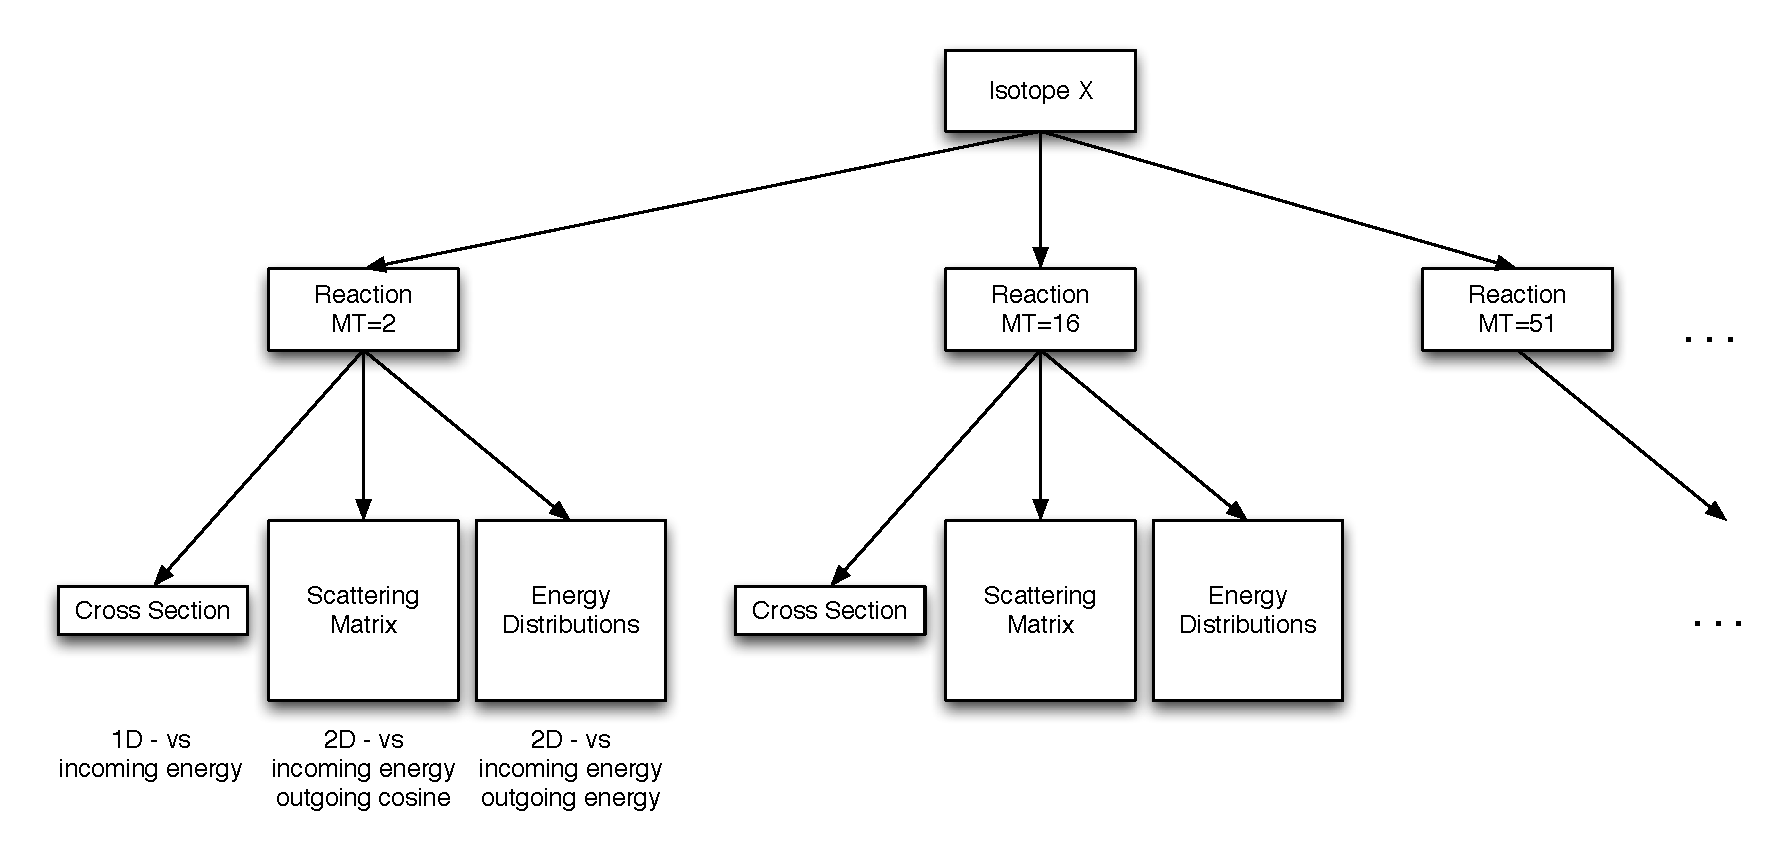
\includegraphics[width=0.8\textwidth]{graphics/data_levels.eps}
     \caption{Hierarchy in ACE formatted neutron data libraries.  \label{data_levels}}
\end{figure}

Many Monte Carlo codes read ACE formatted data rather than the original ENDF file.  ACE stands for ``a compact ENDF'' and strips out a lot of the extra information unnecessary for neutron transport.  As Figure \ref{data_levels} shows, ACE files not only contain cross sections, but also angle and energy distributions used in scattering and fission.  ENDF assigns a number to each type of reaction called the \emph{MT} number.  Table \ref{MT_numbers}, taken from a LANL website, shows the major numbers \cite{MTnums}.  It can clearly be seen that there are many reactions a neutron can undergo, most of which have very energy strong dependance.  Most of the complexity in modeling nuclear reactors comes from the fact that the data needed to model neutrons is very complicated.  It may be the most important part of the simulation, it is what ties the calculations to reality.  If inaccurate data is used, the results will not have any physical meaning, and the simulation becomes a mathematical exercise. 

%%%%%%%%%%%%%%%%%%%%%%%%%%%%%%
\subsection{Neutron Transport}

Now that the events which can happen to neutrons have been outlined, we will move to describing the neutron population itself.  Since the neutron population in reactors is large, on the order of $10^{XXX}/\mathrm{cm}^3$, and the neutrons themselves have very small radii, about $1.75\times10^{-17}$ cm, the distribution of neutrons can be treated as an continuum.  We will eventually derive the \emph{neutron transport equation}, which is a linearized version of the Boltzmann transport equation.  It is linear since it is assumed that neutrons do not interact with each other.  This is usually a good assumption in normal matter since the neutron density present in reactors is many orders of magnitude smaller than the material density and neutrons are much more likely to interact with it than each other.  

Other than eliminating neutron self interaction, there are a handful of other assumptions that go into the equation that will hold true for the rest of the derivations.  One that follows veery closely is that neutrons are assumed to be points in space, so even at very high densities they sill will not interact with each other, and later when we start to discretize spaces, neutrons cannot be in more than one unique volume by overlapping.  The next assumption is that any relativistic effects are negligible.  The energies of importance in reactor physics are below 10MeV, which is about where they start to become non-negligible for neutrons.  Since neutrons are neutral and have long interaction distances compared to their radii, they are also assumed to move in straight lines between collisions.  Materials are also assumed to be in thermal equilibrium and have isotropic properties.  Materials like graphic and water do not have isotropic properties when it comes to scattering, however.  As will be explained later, this can be corrected by adjusting the scattering kernel.

\subsubsection{Neutron Balance Equation}

\begin{figure}[h!] 
  \centering
    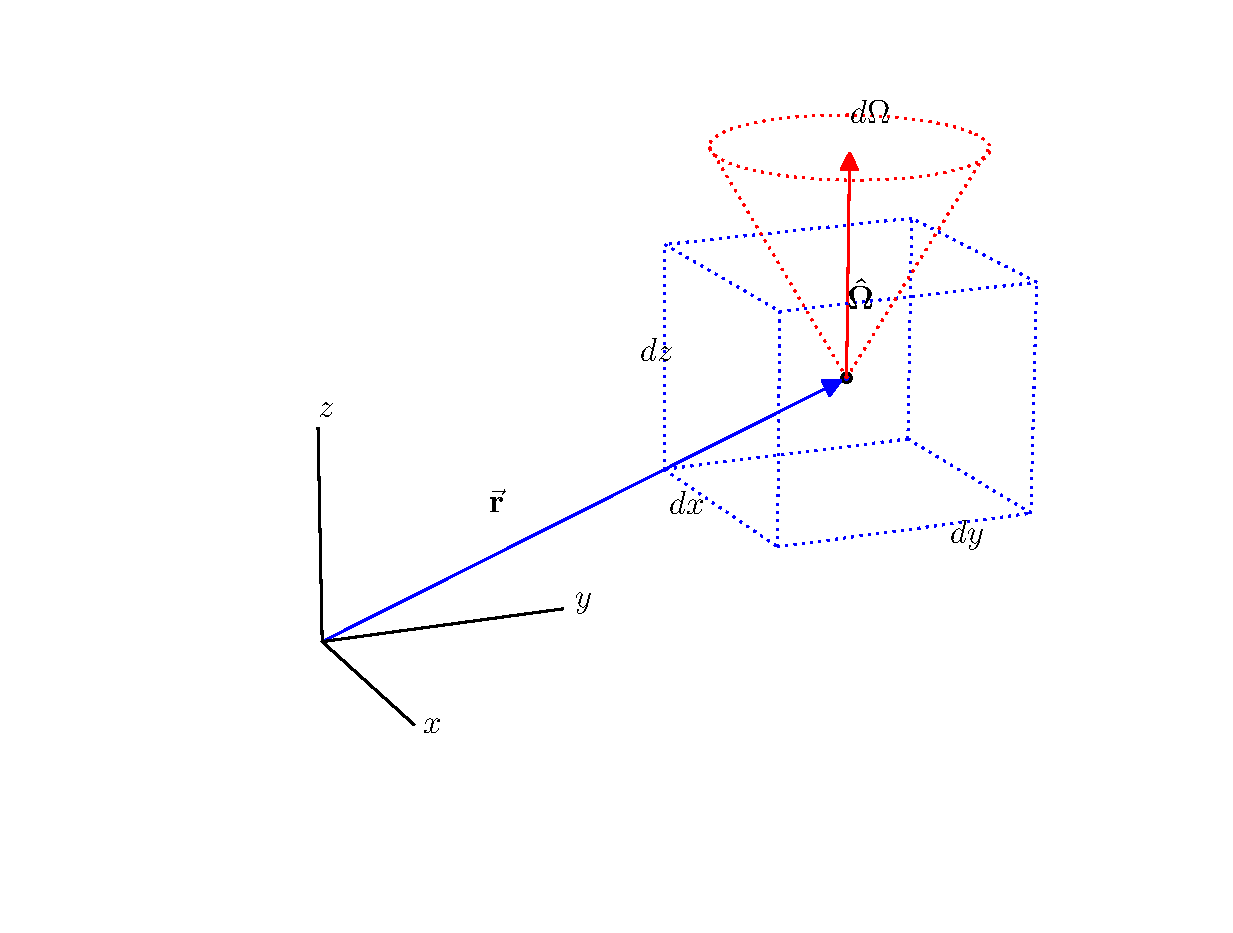
\includegraphics[width=0.8\textwidth,trim= 0cm 2.5cm 0cm 0cm]{graphics/diff_balance.eps} 
     \caption{The differential volume of the neutron balance equation. \label{diff_volume}}
\end{figure}

Before any explicit terms need to defined to capture the necessary physics of the transport problem, a balance equation can be written for a differential volume.  This equation simply describes the amount of neutrons entering and exiting a infinitesimally small volume and their difference being equal to the rate of change of neutrons in the volume.  We know about the reactions that neutrons can undergo, and we know they move through material, so we should have  enough information the write this abstract equation. Figure \ref{diff_volume} shows an illustration of the differential volume.

\begin{equation}
\footnotesize
\label{NBE}
\begin{array}{c}
\mathrm{rate\:of\:change} = (\mathrm{neutrons\:in}) - (\mathrm{neutrons\:out}) \\
\\
\frac{\partial n}{\partial t} = ( \mathrm{movement\:in} + \mathrm{source} + \mathrm{scatter\:in}) - ( \mathrm{movement\:out} + \mathrm{disappearance} + \mathrm{scatter\:out})
\end{array}
\end{equation}

Now that this equation has been written, we can start to explicitly define the terms.  One quantity has already been touched upon - the neutron density.  The neutron density is the fundamental quantity in reactor physics.  This is shown in \eqref{NBE} as $n$, but in the subsequent sections its dependencies will be elaborated on, as will all other dependencies.


\subsubsection{Neutron Distribution Function}

The \emph{neutron distribution function} simply describes the number of neutrons present in each differential quantity it represents.  The most detailed version is differential in space, angle, energy (or velocity), and time, and has inverse units of these dimensions.  In other words, it describes a density in each of it components.  In the subsequent derivations, the spatial, or position vector will be represented by $\boldsymbol{\vec{r}}$, the angular vector by $\boldsymbol{\hat{\Omega}}$, energy by $E$, and time by $t$.  The angle vector is a unit vector that specifies direction only, not magnitude.  It is easiest to express the directional vector as a unit vector in spherical coordinates $(\theta, \phi)$, the polar angle and the azimuthal angle, respectively.  Their cartesian projections are given by \eqref{ang_cart} and shown in Figure \ref{ang_relations}.

\begin{equation}
\label{ang_cart}
\begin{split}
\Omega_x &= \sin \theta \sin \phi  \\
\Omega_y &= \sin \theta \cos \phi \\
\Omega_z &= \cos \theta = \mu
\end{split}
\end{equation}

\begin{figure}[h!] 
  \centering
    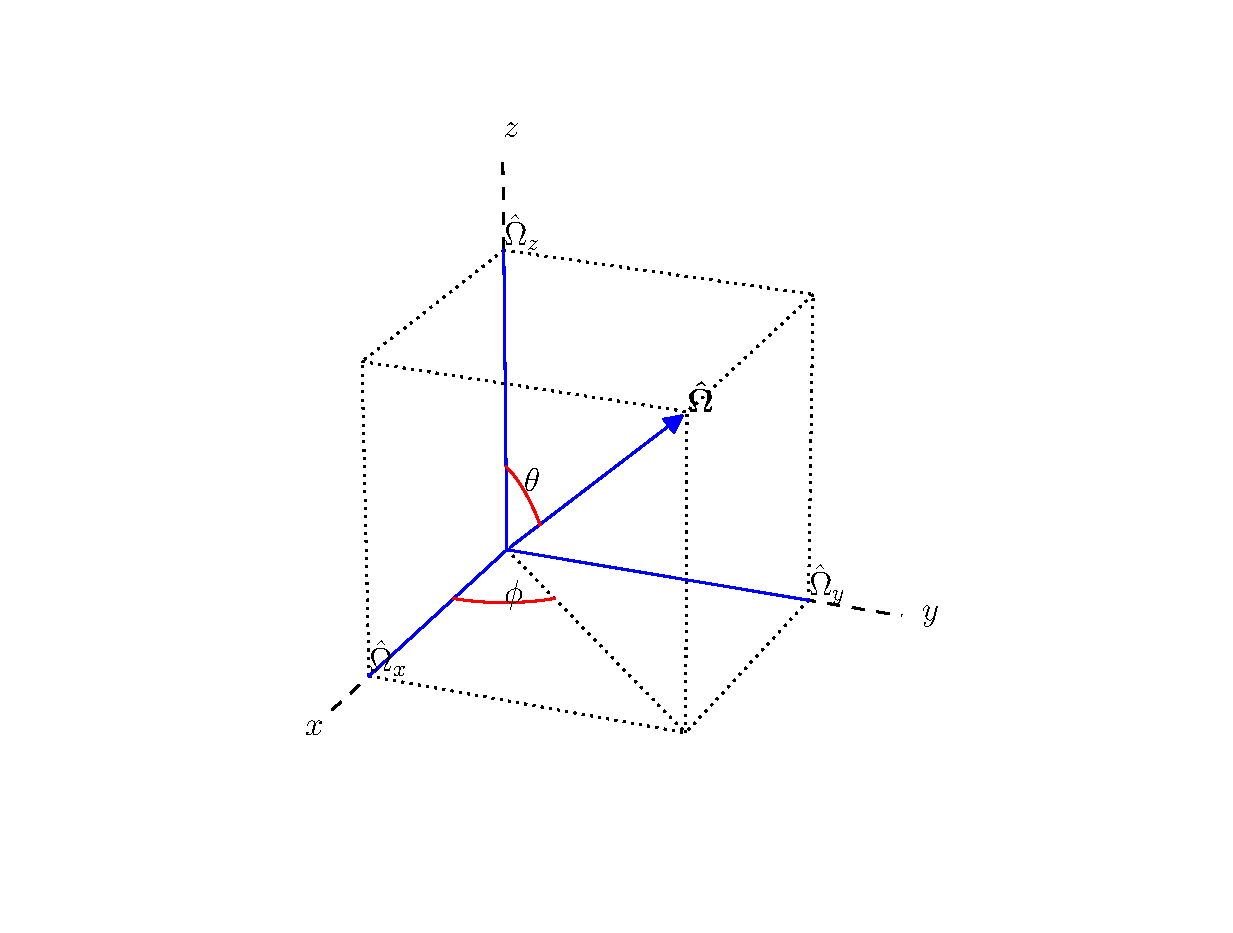
\includegraphics[width=0.8\textwidth , trim= 0cm 2.5cm 0cm 0cm]{graphics/ang_relation.eps} % trim = l b r t
     \caption{The cartesian projections of the directional vector. \label{ang_relations}}
\end{figure}

Like any continuous distribution, it must be integrated over to calculate any quantities.  If we define the $i$th moment of the distribution according to \eqref{NDF_moments}, then the $0$th moment would be the population and the $1$st moment would be the mean.

\begin{equation}
\label{NDF_moments}
M_i = \int_{-\infty}^{\infty} n(x)  x^{i} dx
\end{equation}

For example, if we are given a neutron distribution which has no time dependence, $n(\boldsymbol{\vec{r}},\boldsymbol{\hat{\Omega}},E)$, and wanted to calculate the total number of neutrons present in a volume V, we would calculate this number by \eqref{NDF_sample}, whereas if we wanted to know the average energy, we would do this by \eqref{NDF_avg}.

\begin{equation}
\label{NDF_sample}
N_V = \int_0^\infty \int_{\boldsymbol{\hat{\Omega}}} \int_{V} n(\boldsymbol{\vec{r}},\boldsymbol{\hat{\Omega}},E) dV d\boldsymbol{\hat{\Omega}} dE
\end{equation}

\begin{equation}
\label{NDF_avg}
\bar{E} = \int_0^\infty \int_{\boldsymbol{\hat{\Omega}}} \int_{V} E n(\boldsymbol{\vec{r}},\boldsymbol{\hat{\Omega}},E) dV d\boldsymbol{\hat{\Omega}} dE
\end{equation}

\subsubsection{Reaction Rates}

A \emph{reaction rate} is the rate at which a certain reaction is happening in a volume.  If we go to a pulse-type scenario once more, we have $N_\mathrm{p}$ particles which travel at speed $v$ in one direction.  If $\Sigma$ is the interaction probability per unit length, multiplying it by the speed gives the probability of interaction per second, or the \emph{collision rate}.  Since there are $N$ particles, multiplying the rate by it gives the overall reaction rate, $N_\mathrm{p} v \Sigma$, of the pulse in an infinite medium.  If $N$ is now substituted for the neutron distribution function instead of a pulse, the expression now becomes the reaction rate per distribution differential, or the \emph{reaction rate density}.  This expression is shown in \eqref{RR} and is the first building block of the \emph{neutron balance equation}.

\begin{equation}
\label{RR}
R(\boldsymbol{\vec{r}},\boldsymbol{\hat{\Omega}},E,t)  = v(E) n(\boldsymbol{\vec{r}},\boldsymbol{\hat{\Omega}},E,t) \Sigma(\boldsymbol{\vec{r}},E)
\end{equation}

If we assume there is only one energy, $E_0$ and one direction, $\hat{x}$, and integrate over the constant dimensions of this equation, as shown in \eqref{1d_diff}, we get an expression for the reaction rate in an infinitesimal slice dx.  $A$ is the area perpendicular to the direction of motion where the neutron population is nonzero.


\begin{equation}
\label{1d_diff}
\int_A \int_{\boldsymbol{\hat{\Omega}}} \int_0^{\infty}  dE d\boldsymbol{\hat{\Omega}} dxdydz  v(E) n(\boldsymbol{\vec{r}},\boldsymbol{\hat{\Omega}},E,t) \Sigma(\boldsymbol{\vec{r}},E) \delta(E-E_0) \delta(\boldsymbol{\hat{\Omega}}-\hat{x})  = v \Sigma A n(x)dx 
\end{equation}

This is effectively the loss term for a beam in the $\hat{x}$ direction, and if we set it as such, we recover the beam-type expression \eqref{recover_beam}, which is equivalent to \eqref{pop_diff}.  

\begin{equation}
\label{recover_beam}
dn(x) = - v \Sigma A n(x)dx  \qquad \Rightarrow \qquad  \frac{dI(x)}{dx}= - \Sigma I
\end{equation}


\subsubsection{Angular and Scalar Flux}

Since the reactions rate density is dependent on the cross section and the velocity multiplied by the neutron distribution, this quantity is redefined as the \emph{angular flux} as shown in \eqref{ang_flux}.  Flux meaning that it represents a rate at which particles are passing through a surface, and angular meaning that it is differential in angle.  Again, since the reactions rates depend on this quantity, the neutron transport problem is usually written in terms of the angular flux, which is then solved for instead of the neutron distribution.

\begin{equation}
\label{ang_flux}
\psi(\boldsymbol{\vec{r}},\boldsymbol{\hat{\Omega}},E,t) = v(E) n(\boldsymbol{\vec{r}},\boldsymbol{\hat{\Omega}},E,t)
\end{equation}

Scattering and neutron movement have angular dependence, but reaction cross sections do not, so the reactions can be written in terms of angular flux which has been integrated over all angles, or the \emph{scalar flux} or simply the \emph{flux}.  The relation between the two fluxes is show in \eqref{scalar_flux}.  This is usually the most interesting quantity in reactor physics since the reactor power profile is directly proportional to it.  The reaction rate for a reaction $i$ is shown in \eqref{scalar_flux_RR}.

\begin{equation}
\label{scalar_flux}
\phi(\boldsymbol{\vec{r}},E,t) = \int_{4\pi} \psi(\boldsymbol{\vec{r}},\boldsymbol{\hat{\Omega}},E,t)
\end{equation}

\begin{equation}
\label{scalar_flux_RR}
 R_i(\boldsymbol{\vec{r}},E,t) = \int_{4\pi} \Sigma_i(\boldsymbol{\vec{r}},E) \psi(\boldsymbol{\vec{r}},\boldsymbol{\hat{\Omega}},E,t) = \Sigma(\boldsymbol{\vec{r}},E) \int_{\boldsymbol{\Omega}} \psi(\boldsymbol{\vec{r}},\boldsymbol{\hat{\Omega}},E,t) = \Sigma(\boldsymbol{\vec{r}},E) \phi(\boldsymbol{\vec{r}},E,t)
 \end{equation}
 
 From \eqref{NBE} we can see that the time derivative is in terms of the neutron density, not the angular flux.  Since reaction rates are proportional to angular flux, the balance equation will be written in terms of it.  This mean that the time dependent term must be transformed to angular flux by multiplying and dividing it by the velocity as shown in \eqref{time_depedent_flux}.

\begin{equation}
\label{time_depedent_flux}
\frac{\partial }{\partial t}n(\boldsymbol{\vec{r}},\boldsymbol{\hat{\Omega}},E,t) = \frac{\partial }{\partial t}  \frac{v(E)}{v(E)} n(\boldsymbol{\vec{r}},\boldsymbol{\hat{\Omega}},E,t) =  \frac{\partial }{\partial t}  \frac{\psi(\boldsymbol{\vec{r}},\boldsymbol{\hat{\Omega}},E,t)}{v(E)} = \frac{1}{v(E)} \frac{\partial }{\partial t}\psi(\boldsymbol{\vec{r}},\boldsymbol{\hat{\Omega}},E,t)
\end{equation}

\subsubsection{Scattering}

Scattering is highly dependent on angle and energy and requires as more detailed cross section than disappearance reactions.  Elastic scattering has a fixed relation between outgoing energy and angle, but inelastic scattering does not.  Scattering moves a neutrons energy and angle, so to be completely general in describing it, the cross section is assumed to not only ne dependent on incoming energy like all other cross sections, but also on outgoing energy, incoming angle, and outgoing angle.  Since two quantities are being related before and after a scattering event, the scattering cross section is considered \emph{doubly differential} and is sometimes called the \emph{scattering kernel} whereas the integrated value which only depends on incoming energy is called the scattering cross section.   An expression for the scattering kernel is shown in \eqref{scattering_DD_xs} with the incoming values primed.

\begin{equation}
\label{scattering_DD_xs}
\Sigma_s = \Sigma_s(E^\prime \rightarrow E,\boldsymbol{\hat{\Omega}}^\prime \rightarrow \boldsymbol{\hat{\Omega}})
 \end{equation}

There is a practical reason for separating scattering into a total cross section that describes its likelihood, or probability of a neutron entering the reaction, and a kernel that describes how it exits.  In a Monte Carlo simulation, the cross section is used to determine \emph{whether} scattering happens rather than \emph{how} it happens.  The scattering kernel is only used if a neutron has already been determined to scatter.  This is also shown in the expressions for the scattering in a differential volume.  The cross section is used as the removal of a neutron from a particular energy, whereas the kernel is used to determine from which other energies and angles a neutron is scatter \emph{into}.  This can be seen in \eqref{scattering_DD_xs}.  If the outgoing energy and angle are held constant, the quantity is the probability which other angles and energies scatter into it.

Using these two quantities, source and loss terms can be written for scattering.  The expression for loss uses the cross section, shown in \eqref{scattering_loss}, and the kernel is used in what is often called the \emph{scattering source} term, shown in \eqref{scattering_source}.  The source term need to be integrated over all other energies $E^\prime$ and angles, $\boldsymbol{\hat{\Omega}}^\prime$, which neutrons can scatter into energy $E$ and angle $\boldsymbol{\hat{\Omega}}$.

\begin{equation}
\label{scattering_loss}
R_{s, \mathrm{loss}}( \boldsymbol{\vec{r}},\boldsymbol{\hat{\Omega}},E,t ) = \Sigma_s (\boldsymbol{\vec{r}},E) \psi(\boldsymbol{\vec{r}},\boldsymbol{\hat{\Omega}},E,t)
 \end{equation}
 
 \begin{equation}
\label{scattering_source}
R_{s, \mathrm{source}}(\boldsymbol{\vec{r}},\boldsymbol{\hat{\Omega}},E,t) = \int_0^\infty  \int_{4\pi} \Sigma_s(E^\prime \rightarrow E,\boldsymbol{\hat{\Omega}}^\prime \rightarrow \boldsymbol{\hat{\Omega}}) \psi(\boldsymbol{\vec{r}},\boldsymbol{\hat{\Omega}}^\prime,E^\prime,t) d\boldsymbol{\hat{\Omega}}^\prime dE^\prime
 \end{equation}
 
 \subsubsection{Fission Source}

The nuclear chain reaction is sustained by fission reactions producing neutrons, so it is essential to model it in any material that has fissionable isotopes.  There are three determining factors for the fission source.  The first is the fission reaction rate, which is represented by the flux multiplied by the fission cross section.  The second is the fission spectrum, which is represented by $\chi$.  Neutrons born from fission are not emitted at a single energy, and the fission spectrum describes the probability for a neutron to be emitted at a certain energy.  The energy spectrum is weakly dependent of the incoming neutron energy, which higher incoming energies producing more higher energy neutrons.  This dependence only starts making a significant difference in spectrum shape at energies above 10MeV, higher than energies usually seen in a reactor.  This is why the fission spectrum is usually treated as being independent of incoming neutron energy.  The spectra of uranium-235 and plutonium-239 for fission induced by a 0.5 MeV neutron are shown in Figure \ref{fiss_spec}, and it can be seen that plutonium-239 produces more high energy neutrons.  The last parameter is the average number of neutrons emitted in a fission event, or the \emph{fission yield}, represented by $\nu$, and is relatively flat until about 1MeV, as was shown in Figure \ref{nu_compare}.  Since 1MeV is within the typical energy range present in nuclear reactions, it is treated as a function of energy.

\begin{figure}[h!] 
  \centering
    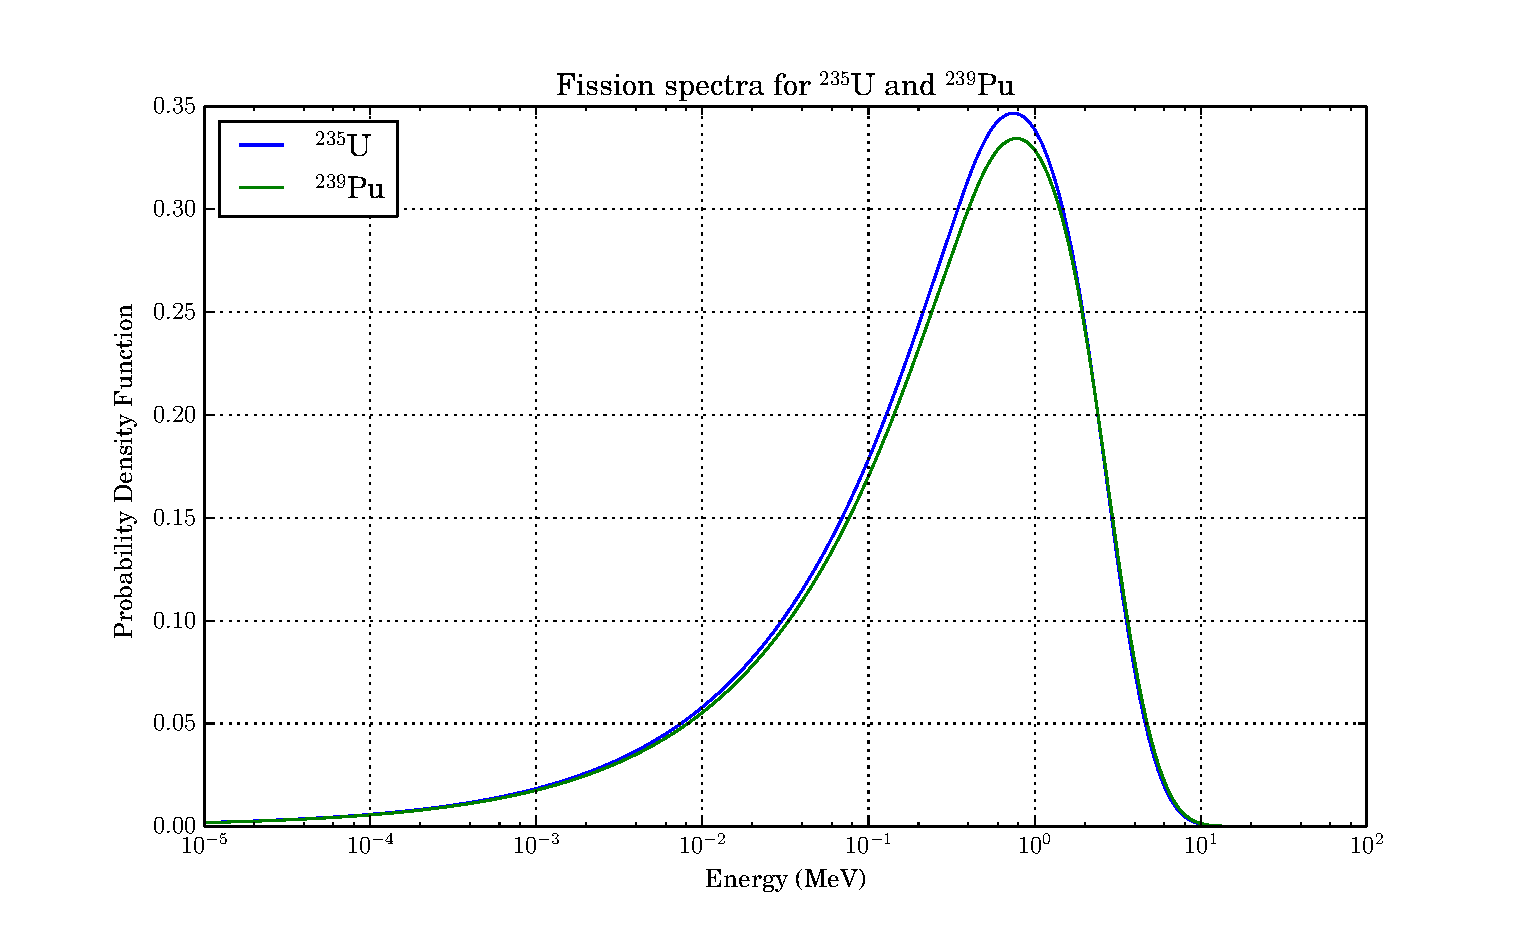
\includegraphics[width=0.8\textwidth ]{graphics/fiss_spec.eps} 
     \caption{The prompt fission spectrum for uranium-235 and plutonium-239. \label{fiss_spec}}
\end{figure}

To write an expression for the fission source, or the number of fission neutrons born in energy $E$, we must know the number of neutrons born from fission at all energies.  Once this is known, it is multiplied by the fission spectrum to select the fraction that will be in energy $E$.  The expression for the fission source is shown in \eqref{fiss_source}.

\begin{equation}
\label{fiss_source}
\frac{\chi(E)}{4\pi} \int_0^\infty  \int_{4\pi}   \nu(E^\prime) \Sigma_f(\boldsymbol{\vec{r}},E^\prime) \psi(\boldsymbol{\vec{r}},\boldsymbol{\hat{\Omega}}^\prime,E^\prime,t) d\boldsymbol{\Omega}^\prime  dE^\prime = \frac{\chi(E)}{4\pi} \int_0^\infty   \nu(E^\prime) \Sigma_f(\boldsymbol{\vec{r}},E^\prime) \phi(\boldsymbol{\vec{r}},E^\prime,t)  dE^\prime
 \end{equation}


\subsubsection{Streaming}

So far all that has been  touched on is how neutrons within a volume move in angle and energy or are removed outright.  Now we will go over how they move in space, and to do this we consider a surface $S$ around our differential volume.  We want to find an expression for the net number of neutrons passing through this surface and this will be our net leakage term (incoming minus outgoing).  The angular neutron flux describes the number of neutrons crossing a differential surface at angle $\boldsymbol{\hat{\Omega}}$, but in order to perform any vector operations on it, we must multiply it by the unit vector.  We can then write and expression for the leakage by performing a surface integral over the current and surface normal's dot product, shown in \eqref{leakage_surface}.

\begin{equation}
\label{leakage_surface}
\mathrm{Leakage} = \int_S ds \cdot \boldsymbol{\hat{\Omega}} \psi(\boldsymbol{\vec{r}},\boldsymbol{\hat{\Omega}},E,t)
\end{equation}
 
 We can turn this into a volume integral by applying the divergence theorem, shown in \eqref{div_theorem}.  If the volume of interest is shrunk to an infinitesimal volume and we switch the order of the dot product, we come to an expression that can be used in the balance equation.  This expression, shown in \eqref{streaming}, is often called the \emph{streaming} term, since it describes the net movement of neutrons into the differential volume due to their physical movement.
 
\begin{equation}
\label{div_theorem}
\int_S ds \cdot \boldsymbol{\hat{\Omega}} \psi(\boldsymbol{\vec{r}},\boldsymbol{\hat{\Omega}},E,t) = \int_V dV \nabla \cdot \boldsymbol{\hat{\Omega}}  \psi(\boldsymbol{\vec{r}},\boldsymbol{\hat{\Omega}},E,t)
\end{equation}

\begin{equation}
\label{streaming}
 \lim_{V\to dV} \int_V dV \nabla \cdot \boldsymbol{\hat{\Omega}}  \psi(\boldsymbol{\vec{r}},\boldsymbol{\hat{\Omega}},E,t) =  \boldsymbol{\hat{\Omega}}  \cdot \nabla\psi(\boldsymbol{\vec{r}},\boldsymbol{\hat{\Omega}},E,t) 
 \end{equation}
 

\subsubsection{Neutron Transport Equation}

Now all the terms of \eqref{NBE} have been explicitly defined.  Substituting them all in yields \eqref{NTE}, the \emph{neutron transport equation}, written here with the neutron sinks on the left side and the neutron sources on the right side.  An additional external source term, $S_{\mathrm{external}}$, has been added to account for any sources not induced by the neutron flux itself, i.e. external sources.  

\begin{equation}
\label{NTE}
\begin{split}
\frac{1}{v(E)} \frac{\partial }{\partial t}\psi(\boldsymbol{\vec{r}},\boldsymbol{\hat{\Omega}},E,t) &+  \\
\boldsymbol{\hat{\Omega}}  \cdot \nabla \psi(\boldsymbol{\vec{r}},\boldsymbol{\hat{\Omega}},E,t) &+ \\
\Sigma_t(\boldsymbol{\vec{r}},E) \psi(\boldsymbol{\vec{r}},\boldsymbol{\hat{\Omega}},E,t) & \\
& =  \\
& \quad \int_0^\infty  \int_{4\pi} \Sigma_s(E^\prime \rightarrow E,\boldsymbol{\hat{\Omega}}^\prime \rightarrow \boldsymbol{\hat{\Omega}}) \psi(\boldsymbol{\vec{r}},\boldsymbol{\hat{\Omega}}^\prime,E^\prime,t) d\boldsymbol{\Omega}^\prime dE^\prime  \\
&+ \frac{\chi(E)}{4\pi} \int_0^\infty  \int_{4\pi}   \nu(E^\prime) \Sigma_f(\boldsymbol{\vec{r}},E^\prime) \psi(\boldsymbol{\vec{r}},\boldsymbol{\hat{\Omega}}^\prime,E^\prime,t) d\boldsymbol{\Omega}^\prime  dE^\prime\\
& + S_{\mathrm{external}}
\end{split}
 \end{equation}
 
 The neutron transport equation in this form is an integro-differential equation since it has both derivates and integrals in it.  It's spatial parts are differential, whereas its angular and energy parts are integral.  It is linear and relatively easy to solve for simple geometries and reaction parameters.  The complexity in solving it comes from the complex energy dependence of the reaction parameters and the large and complex domains over which it must be solved in order to capture all the relevant physics.  The reaction parameters can span more then 12 orders of magnitude, from $1\times 10 ^{-11}$ to $1\times 10 ^{1}$ MeV and above, and the geometries involved can include millions of individual material regions with many different mixtures of material within them.
 
 \subsubsection{Time Independent Neutron Transport Equation}

In most situations, the equilibrium state of the neutron population is of interest.  By setting all time derivates to zero, \eqref{NTE} becomes the time-independent neutron transport equation shown in \eqref{time_ind_NTE}.  Another parameter has been introduced, the effective multiplication factor, $k_\mathrm{eff}$, which was described earlier using the seven factor formula.  It is introduced here since by forcing the time derivates to be zero, it is implied that the multiplication factor must be equal to one.  The material and geometric properties of a problem may say otherwise, however, and failing to divide the fission source by the effective multiplication factor could make time independent equation inconsistent.  Of course, there will be no inequality if the source and sink terms are actually balanced and $k_\mathrm{eff}$ calculated from \eqref{NTE} is one.

\begin{equation}
\label{time_ind_NTE}
\begin{split}
\boldsymbol{\hat{\Omega}}  \cdot \nabla \psi(\boldsymbol{\vec{r}},\boldsymbol{\hat{\Omega}},E,t) &+ \\
\Sigma_t(\boldsymbol{\vec{r}},E) \psi(\boldsymbol{\vec{r}},\boldsymbol{\hat{\Omega}},E,t) & \\
& =  \\
& \quad \int_0^\infty  \int_{4\pi} \Sigma_s(E^\prime \rightarrow E,\boldsymbol{\hat{\Omega}}^\prime \rightarrow \boldsymbol{\hat{\Omega}}) \psi(\boldsymbol{\vec{r}},\boldsymbol{\hat{\Omega}}^\prime,E^\prime,t) d\boldsymbol{\Omega}^\prime dE^\prime  \\
&+ \frac{1}{k_{\mathrm{eff}}}\frac{\chi(E)}{4\pi} \int_0^\infty  \int_{4\pi}   \nu(E^\prime) \Sigma_f(\boldsymbol{\vec{r}},E^\prime) \psi(\boldsymbol{\vec{r}},\boldsymbol{\hat{\Omega}}^\prime,E^\prime,t) d\boldsymbol{\Omega}^\prime  dE^\prime\\
& + S_{\mathrm{external}}
\end{split}
 \end{equation}
 

\section{Discrete Methods}

The usual method in solving continuous differential and integral equations on a computer is to discretize the domain over which it is being solved.  This can be applied to the neutron transport equation as well.  Since energy is involved in integrals in the neutron transport equation, it can be discretized by integrating over set boundaries and treating the reaction parameters as constant within them.  The same method can be applied to them angular dependence.   The simplest way of discretizing the geometry is to voxelize the domain, laying down a uniform grid in every dimension and treating the material within each voxel as being uniform.  Discrete geometry representation is and area where an lot of error can occur since it is three dimensional and scales can range from millimeters to hundred of meters. 

derivations?  moments, diffusion, SN?

Although discrete methods are readily mapped to computer hardware and execute quite fast, there are drawbacks and limitations in using them.  The biggest drawback is that they're accuracy greatly depends and the discretization methods used.  MORE.

\section{Monte Carlo}

The Monte Carlo method takes a different approach in mapping the transport problem to a computer.  Instead of the neutron population being continuous and the spatial, angular, and energy dimensions being discretized, it leaves the dimensions continuous and discretizes the neutron population!   Quantities of interested are then determined by integrating over the neutron population!   This way of integrating the neutron transport equation can be thought of as integrating it ``sideways.''   Deterministic approaches integrate it by discretizing the dimensions and ensuring consistency of the transport equation between the discrete points.  This is the ``standard'' way of integrating the transport equation.  In the Monte Carlo method, the discretized neutron ``shoots through'' the transport equation many times, sweeping out the entire phase space, effectively integrating it when a sum is done over the individual neutron realizations, or \emph{histories}.  It is important to note that the Monte Carlo method does not actually solve the transport equation, per se, but rather is able to \emph{estimate} the solution very well.

The Monte Carlo approach makes a physically analogous ``experiment'' on a computer.  A computer thread ``sits on top'' of a neutron as it makes a \emph{random walk} through the geometry.  The computer thread uses pseudo-random numbers to sample probability distributions that describe the interactions the neutron makes as it travels.  All the assumptions that went into deriving the neutron transport equation still hold, most importantly that neutrons travel in straight lines between interactions, the neutrons are points, and they do not interact with each other.  The other assumption is that interactions happen instantaneously and at a point, i.e. they do occur over a distance.  It is very important how surface crossing detected in the simulation since this is what changes the material data where the probability distributions come from.  WARP, in its current state, uses the traditional form of surface detection and material updates, ray tracing, the details of which will be discussed in Section \ref{sec:prelim}.  When a neutron is sampled to cross a surface, it is placed on the boundary, the material data is updated, and the interaction distance is sampled again with the neutron traveling in the same direction.  Figure \ref{random_walk} shows a cartoon of a random walk of a neutron born in the center of a cube.  The line colors represent a neutron sampling a specific material, the red ``X'' represents an absorption (walk termination), and the green ``X'' represents a surface crossing.

\begin{figure}[h!] 
  \centering
    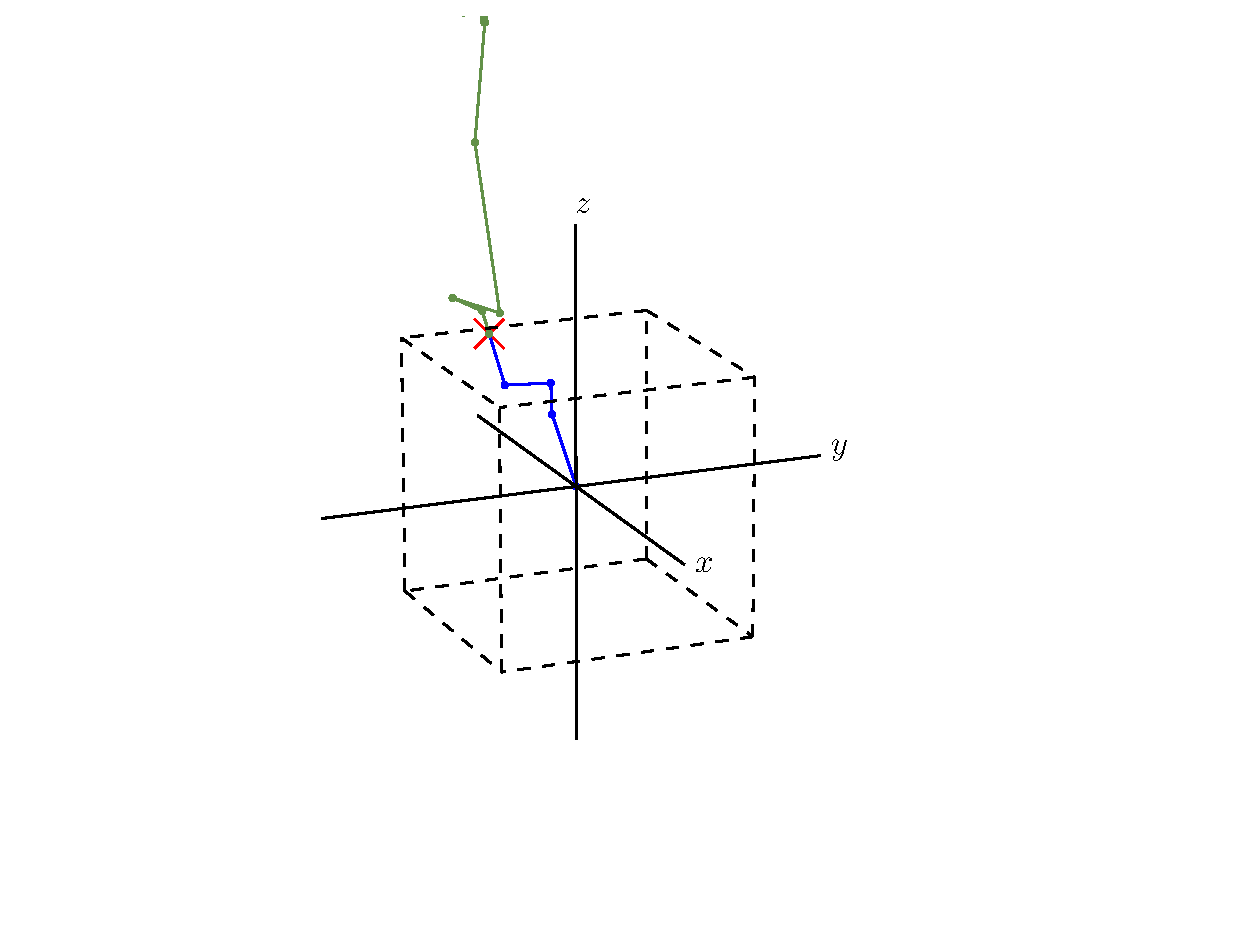
\includegraphics[width=0.8\textwidth,trim= 0cm 2.5cm 0cm 0cm]{graphics/random_walk_accepted.eps}
     \caption{The Monte Carlo random walk process. \label{random_walk}}
\end{figure}

There are advantages in using the Monte Carlo method for neutron transport, some of which have been mentioned.  The first and foremost is that it that very few assumptions must be done to the physics and the geometry of the problem. Paraphrasing Forrest Brown when he spoke at the Supercomputing in Nuclear Applications and Monte Carlo conference on October 30th, 2013 in Paris,  the only reason people use Monte Carlo methods is that they are able to produce physically accurate results and are trusted to so so.  Anyone developing Monte Carlo code should not abuse this trust and must put accuracy first and foremost in their implementations.

There are considerable drawbacks to using Monte Carlo as well; primarily convergence rates and silent inaccuracies.  Since it is a statistical calculation, it is bound by statistical laws which dictate that the error in Monte Carlo calculations reduces as $1/\sqrt{N}$, where N is the number of histories performed.  Also, since geometries can be large, very small but very influencing volumes can be missed by the neutron random walk if the number of histories is not large enough.  The estimated statistical error may be low at $N$ histories, but there is a chance the entire phase space has not yet been sufficiently sampled to produce accurate results.  Deterministic methods would not have this problem since there will be a discretized point in this small volume, and it will contribute to the overall calculation.  The slow convergence rate can be combated by using parallel computing, however.  Requiring that neutrons do not interact with each other was an assumption that went into deriving the neutron transport equation, and can be exploited in Monte Carlo simulations.  Since each neutron history is completely independent, histories can be run completely in parallel without communication until the results are combined at the end of the simulation.  This leads to very good scaling of parallel calculations, which can be used to reduced run times of large problems to acceptable values.

\subsection{Statistics}

To understand how the Monte Carlo method performs this integration, simple equations and derivations and such as calculating $\pi$ can be done.   First, given a continuous random variable $x$ that follows the probability distribution $P$, the mean value can be calculated by taking the first moment as was shown in \eqref{NDF_moments} and is reproduced in \eqref{int_mean}.  But we are interested in determining the mean from a set measurements rather than the underlying distribution.  If we have $N$ independent measurements of quantity $x$, this is simply taking the arithmetic mean, as shown in \eqref{arith_mean}.

\begin{equation}
\label{int_mean}
\mu = \int_{-\infty}^{\infty} x P(x) dx
\end{equation}

\begin{equation}
\label{arith_mean}
\bar{X}_N = \frac{1}{N} \sum_i^N x_i
\end{equation}

The shape of the distribution about the mean is important as well, since it quantifies the uncertainty.  The variance can be computed by performing the central second moment on $P$ and estimated by Bessel's Correction on the standard variance estimator \eqref{varience_est}\cite{}.  It is useful that the sample mean can be removed from the sum of the sample squares since this means that only the sample sum and the sum of sample squares need be stored.  The entire sample set does not need to be stored and used to compute the variance at the end when the sample mean is known.

\begin{equation}
\label{varience}
\sigma^2 = \int_{-\infty}^{\infty} x^2 P(x) dx- \mu^2
\end{equation}

\begin{equation}
\label{varience_est}
\sigma_N^2 =  \frac{1}{N-1} \sum_i^N (x_i-\mu)^2 =  \frac{1}{N-1} \left( \sum_i^N x_i^2-N\bar{X}_N^2 \right)
\end{equation}

The law of large number states that \eqref{arith_mean}, the sample mean, will converge to the true mean \eqref{int_mean} in the limit where $N\rightarrow\infty$.  

\begin{equation}
\label{LLN}
Pr\left(\lim_{N\rightarrow\infty} \bar{X}_N = \mu \right) =0
\end{equation}

The rate at which the estimate \eqref{arith_mean} converges to the true mean \eqref{int_mean} comes from the central limit theorem.  Shown in \eqref{CLT}, it states that the distribution of the means of taken from a large set of independent random variables will be normally distributed.  

\begin{equation}
\label{CLT}
\sqrt{N}\left(\left(\frac{1}{N} \sum_i^N x_i \right)-\mu\right) \xrightarrow[]{d} \mathcal{N}(0,\sigma^2)
\end{equation}

In this case, if a large number of measurements are taken, we would like to know how close the mean of a completely independent set measurements will be to the true mean.  In other words, the variance of the mean is desired.  Luckily, this can be estimated with only one measurement instead of directly computing the variance with many measurements.  The Bienaym\'e formula, shown in \eqref{bien}, states that the variance of a sum of uncorrelated random variables is equal to the sum of the variances of the variables.

\begin{equation}
\label{bien}
Var\left(\sum_{i=0}^N x_i \right) = \sum_{i=0}^N Var(x_i)
\end{equation}      


Applying the Bienaym\'e formula and the variance relation show in \eqref{basic_var_scaling} to the sample mean results in an expression for the variance of the mean, $Var(\bar{X}_N)$, in terms of the variance of the sample, $\sigma_N^2$.  This expression is shown in \eqref{sum_var}.  

\begin{equation}
\label{basic_var_scaling}
Var\left(a X \right) = a^2 Var\left( X \right)
\end{equation}

\begin{equation}
\label{sum_var_1}
Var(\bar{X}_i) = Var\left(\frac{1}{N}\sum_{i=0}^N x_i \right) = \frac{1}{N^2} \sum_{i=0}^N Var(x_i) = \frac{N\sigma_N^2}{N^2} =  \frac{\sigma_N^2}{N} 
\end{equation}

\begin{equation}
\label{sum_var}
 \frac{\sigma_N^2}{N} = \frac{1}{N(N-1)} \left( \sum_i^N x_i^2- N\bar{X}_N^2 \right) = \frac{1}{(N-1)} \left( \frac{1}{N} \sum_i^N x_i^2 - \left(   \frac{1}{N} \sum_i^N x_i \right)   \right)
\end{equation}

It should be noted that \eqref{sum_var_1} implies that the standard deviation of the mean always scales as $1/\sqrt{N}$.  This is a blessing and a burden in that it means any calculation will variance of the mean will go to zero, or the sample mean will converge to the true mean, as long it is run long enough and enough samples are collected, but that it will converge as $1/\sqrt{N}$, which is slow.

Since the central limit theorem states that it is normally distributed, we can make use of the well-know properties of the normal distribution, namely the confidence interval.  The normal distribution has well-defined confidence intervals: 68\% of the population will lie within a single standard deviation, $\sigma$, and 95.5\% will lie within $2\sigma$.  From this knowledge, an expression for the realtive error can be written.  The expression for the relative error shown in \eqref{rel_err} is for the 68\% confidence level, and simply needs to be doubled for the 95\% level \cite{MCNP}\cite{jaakko}.

\begin{equation}
\label{rel_err}
\mathrm{Rel. Err.} = \frac{\sigma}{\bar{X}_N} = \frac{1}{\bar{X}_N}\sqrt{\frac{1}{(N-1)} \left( \frac{1}{N}\sum_i^N x_i^2-\bar{X}_N^2 \right)}
\end{equation}

\subsection{Sampling Schemes}

In order to actually transport a neutron across the geometry in a Monte Carlo simulation, a the probability distributions of the reaction types must be sampled in order to produce accurate distributions when the histories are aggregated.  There are two methods that are commonly used to do so; the direct inversion method and the rejection method.  

The \emph{direct inversion} method relies and being able to analytically integrate the probability distribution function (PDF) to create a cumulative distribution function (CDF) and being able to invert it.  The first step is to integrate the PDF to find the CDF, as shown in \eqref{CDF}.

\begin{equation}
\label{CDF}
CDF(x) = \int_0^x PDF(x^\prime) dx^\prime
\end{equation}

Since a PDF must be positive and normalized by definition, the CDF must range from 0 to 1 and increase monotonically.  Setting the CDF equal to a uniformly distributed random number $\xi$ and solving for the value to be sampled yields the sampling scheme.  Figure \ref{direct_samp} shows this graphically.  The CDF describes the probability that a value of a random number $x$ obeying the PDF will be below the value $x$.  Taking an interval gives the probability $x$ will be in the interval, as shown in \eqref{CDF_property1}.  Since the width of inverse CDF is directly proportional to the PDF at the same value of $x$, as shown in \eqref{CDF_property2}, and if $\xi$ is uniformly distributed on [0,1), the interval $\Delta \xi$ will contain a fraction of samples on [0,1) equal to $P( x_1 < x_i < x_2)$.  As the interval is reduced to 0, $P(x_i)= PDF(x)dx = d\xi$ (again, since $\xi$ is uniformly distributed on [0,1), leading to the sampling scheme shown in \eqref{CDF_inversion}.  This method is only useful if the CDF is simple enough to be inverted analytically.

\begin{equation}
\label{CDF_property1}
CDF(x_2) - CDF(x_1) = P( x_1 < x_i < x_2) = \int_{x_1}^{x_2} PDF(x) dx
\end{equation}

\begin{equation}
\label{CDF_property2}
CDF(x_2) - CDF(x_1) = \Delta \xi =  \int_{x_1}^{x_2} PDF(x) dx
\end{equation}

\begin{equation}
\label{CDF_inversion}
 x_i = CDF^{-1}(\xi_i)
\end{equation}

\begin{figure}[h!] 
  \centering
    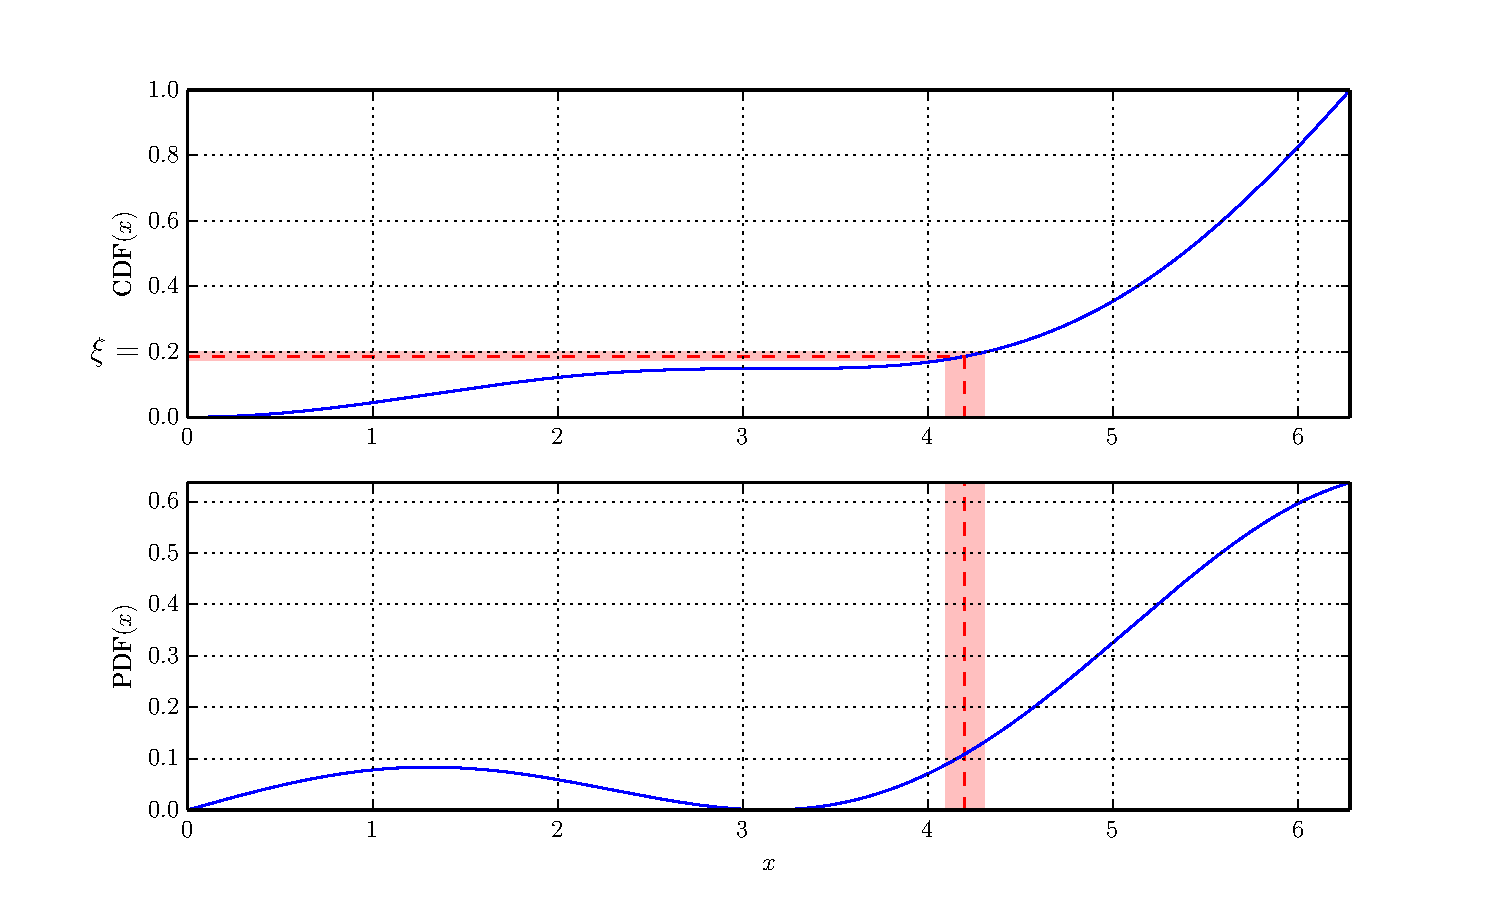
\includegraphics[width=0.8\textwidth]{graphics/direct_samp.pdf}
     \caption{Sampling $PDF(x)=\frac{1}{2\pi^2}(x \cos x - x)$ by the direct inversion method on the domain $(0,2\pi)$. \label{direct_samp}}
\end{figure}

When the CDF is not invertible, the \emph{rejection sampling} method can be used.  It uses a secondary PDF, $f{x}$, that is greater at all points than the PDF to be sampled from and whose CDF is easily inverted.  Since the PDF is normalized, $f(x)$ now corresponds to probabilities greater than one.  This is simply a scaling problem, and the random numbers used to directly sample from it must be uniform on $[0,\int_\mathrm{domain}f(x))$ instead of $[0,1)$.   Then two random numbers are generated.  The first, $\xi_1$ is sampled from a $f(x)$ using a scaled random number as mentioned, and the second, $\xi_2$ is uniformly distributed on $[0,f(\xi_1))$.  If $\xi_2 < PDF(\xi_1)$, the sampled value $(\xi_1)$, is added to the population, else it is \emph{rejected}, or discarded from the population.  The set of accepted values of ${\xi_2}$ will then follow $PDF(x)$.  Figure \ref{rejection_samp} shows an illustration of rejection sampling.

\begin{figure}[h!] 
  \centering
    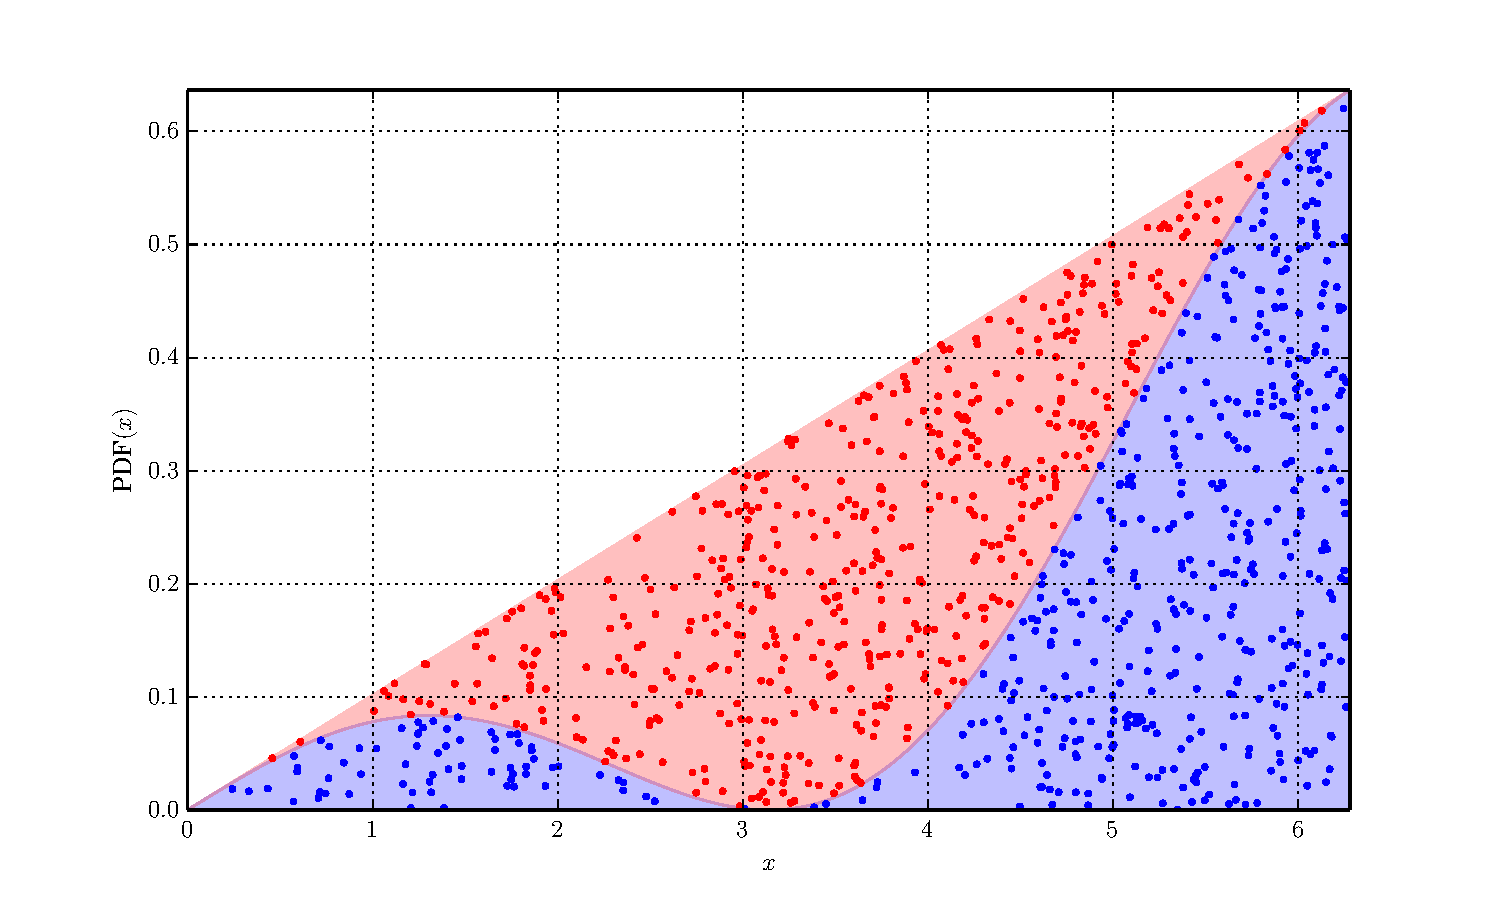
\includegraphics[width=0.8\textwidth]{graphics/rejection_samp.pdf}
     \caption{Sampling $PDF(x)=\frac{1}{2\pi^2}(x \cos x - x)$ by the rejection method on the domain $(0,2\pi)$.  The auxiliary function $f(x)=x/\pi$ and the random number used to sample from it must be on $[0,2\pi)$ instead of $[0,1)$. \label{rejection_samp}}
\end{figure}

Using these two methods of sampling from probability distributions, expressions can be found for every reaction type and transport phenomenon that a neutron undergoes in it's random walk through matter.  The specific schemes are described in the following subsections.

\subsubsection{Cross Section Interpolation}

When a Monte Carlo simulation is referred to as ``Continuous Energy,'' it means that the cross sections are evaluated on the fly at the exact energy the neutron is currently at instead of using a fixed value for a range of energies.  The cross section data is finite, of course, and only includes data at discrete points in energy.  Therefore, interpolation must be performed between the data points.  This is done by linear interpolation.  It assumes that the cross section is a straight line between the surrounding energy points, $E_i$ and $E_{i+1}$, and the interpolated value is calculated using the slope of the line via \eqref{xs_interp}.

 \begin{equation}
\label{xs_interp}
\begin{gathered}
E_i < E < E_{i+1} \\
\sigma(E) = \frac{E-E_i}{E_{i+1}-E_i}(\sigma(E_{i+1})-\sigma(E_i)) + \sigma(E_i)
\end{gathered}
\end{equation}

\subsubsection{Tabular Distribution Interpolation}

For reactions that have any exiting neutrons, like scattering and fission, there are probability tables that specify at what probability certain angles and energies will be emitted.  These tables are typically have a CDF specified in a tabular format.  To sample from these tabular CDFs, a random number $\xi$ is generated.  Again, since the data is discrete, some type of interpolation must be performed to generated a value between the data points.  There are two methods specified in the ENDF format.  The first is histogram interpolation, which is similar to the linear cross section in the previous section.  It assumes the CDF is a line in between the data points, and the interpolated value is calculated to lie on this line.  A tabular PDF is also usually specified, but is not used in the actual computations in this study since the PDF value can be computed from the CDF and doing so reduces the global memory access of a GPU kernel.  Histogram interpolation is shown in \eqref{histo_interp} where $C_{i}$ is the value of the CDF at point $i$.  The outgoing cosine, $\mu^\prime$, is used, but this method can be used to sampled a CDF of any quantity.  $\mu^\prime_i$ represents the corresponding value of $\mu^\prime$ in the table for $P_i$ and $C_i$.

 \begin{equation}
\label{histo_interp}
\begin{gathered}
C_i < \xi < C_{i+1} \\
 \mu^\prime(\xi) = \frac{\xi-C_i}{C_{i+1}-C_i}(\mu^\prime_{i+1}-\mu^\prime_i) + \mu^\prime_i
\end{gathered}
\end{equation}

The second method is called linear-linear interpolation.  Instead of assuming the CDF is linear, it assumes the first derivative (the PDF) is linear over the interval $C_i < \xi < C_{i+1}$.  The linear expression for the PDF as in \eqref{lin_pdf} is substituted into \eqref{CDF_property1} and integrated to $\mu^\prime$.  Again this derivation is shown for $\mu^\prime$, but is valid for any CDF.

\begin{equation}
\label{lin_pdf}
\begin{gathered}
C_i < \xi < C_{i+1} \\
P(\mu^\prime) = \frac{P_{i+1}-P_i}{\mu^\prime_{i+1}-\mu^\prime_i}(\mu^\prime - \mu^\prime_i) + P_i = a \mu^\prime + b
\end{gathered}
\end{equation}

Integration of \eqref{lin_pdf} to $\mu^\prime$ yields \eqref{lin_pdf_int}.  This expression for $CDF(\mu^\prime)$ is set equal to the random number $\xi$ and solved for $\mu^\prime$ to give the interpolation function.

\begin{equation}
\label{lin_pdf_int}
C(\mu^\prime) = C_i  + \int_i^{\mu^\prime} P(\mu^{\prime\prime}) d\mu^{\prime\prime}  = C_i  + \frac{a}{2}(\mu^{\prime 2}-\mu^{\prime 2}_i) + b(\mu^\prime-\mu^\prime_i) = \xi 
\end{equation}

Taking advantage of the relationship between $a$ and $b$, the interpolation function can be simplified to \eqref{lin_lin} \cite{openmc}.

\begin{equation}
\label{lin_lin}
\begin{gathered}
a = \frac{P_{i+1}-P_i}{\mu^\prime_{i+1}-\mu^\prime_i} \qquad , \qquad b = P_i - a \mu^\prime_i \\
\mu^\prime = \mu_1 + \frac{1}{a}\left( \sqrt{P^2_i + 2a(\xi -C_i)} -P_i \right)
\end{gathered}
\end{equation}

Which interpolation method is used is specified in the data on a case-by-case basis.

\subsubsection{Distance To Interaction}

The first step in stochastically transporting a neutron through matter is finding the distance to the next interaction.  The expression for the probability of non-interaction was shown in \eqref{pop_NI}.  The probability of interaction in $dx$ around $x$ is $\Sigma_t dx$.  Therefore the probability of not interacting from 0 to x and then interacting at $dx$ around $x$ is simply the product.  This expression, shown in \eqref{first_col}, is commonly referred to as the \emph{first collision probability}.

\begin{equation}
\label{first_col}
P(x) = \Sigma_t e^{- \Sigma_t  x}
\end{equation}

This expression is simple and can be inverted for direct sampling.  The sampling scheme is shown in \eqref{first_col_samp}.  The expression $1-\xi$ can be replaced with $\xi$ since it is identically distributed.

\begin{equation}
\label{first_col}
CDF(x) = \int_0^x \Sigma_t e^{- \Sigma_t  x^\prime} dx^\prime = 1- e^{- \Sigma_t  x} 
\end{equation}

\begin{equation}
\label{first_col_samp}
x_i=CDF^{-1}(\xi) \qquad \Rightarrow \qquad x_i=\frac{-\ln(1-\xi) }{\Sigma_t}=\frac{-\ln(\xi) }{\Sigma_t}
\end{equation}

The total cross section $\Sigma_t$ is the total macroscopic cross section of the material the neutron is traveling through, i.e. it is the sum of the total macroscopic cross sections of its constituent isotopes as was shown in \eqref{material_sum_xs}.

\subsubsection{Isotope and Reaction Selection}

Now that the neutron has been determined to interact, it must be decided with which isotope it interacts with.  The discrete PDF of this process is shown in \eqref{isotope_selection}, where there are $i$ isotopes in the material each having a total macroscopic cross section $\Sigma_{t,i}$.  The distribution is sampled by generating a uniform random number, $\xi$, on $[0,1)$ and performing a running sum over the individual isotope's total macroscopic cross sections.  When $CDF_i > \xi$, the neutron collision is sampled to happened in isotope $i$.

\begin{equation}
\label{isotope_selection}
PDF_i = \frac{\Sigma_{t,i}}{\Sigma_t} \qquad \Rightarrow \qquad CDF_i = \frac{1}{\Sigma_t } \sum_{n=1}^i \Sigma_{t,n}
\end{equation}

Determining the reaction type is done in a similar fashion, except the number density of the material is no longer a concern since the isotope has already been selected.  Therefore, the running sum of the CDF is done over the isotope $i$'s microscopic cross sections.  Another random number is generated, and when $CDF_k > \xi$, the neutron is sampled to undergo reaction $k$ in isotope $i$.

\begin{equation}
\label{reaction_selection}
PDF_k = \frac{\sigma_k}{\sigma_t} \qquad \Rightarrow \qquad CDF_k = \frac{1}{\sigma_{t} } \sum_{n=1}^k \sigma_{n}
\end{equation}

\subsubsection{Free Gas Treatment}

As stated previously, the data in the cross section libraries are broadened for a certain material temperature.  This is done to account for the effect the nuclides' thermal motion has on the apparent width of resonances even when they are modeled as stationary.  Modeling the targets as stationary is a good approximation when the neutron has much larger larger velocities, but such a model would allow a neutron to scatter down to absolute zero.  In reality, they scatter until they come into thermal equilibrium with the target nuclides.  Once they are in equilibrium, on average they lose the same amount of energy as they gain from scattering events and their population becomes stationary in energy.  

To preserve this collection phenomena, or \emph{thermal peak}, in Monte Carlo simulations, the velocity of the target nuclide must be explicitly modeled.  Elastic scattering is the only interaction that has a neutron in the exit channel at thermal energies, and therefore is the only reaction that needs to consider target velocity.  Fission produces secondary neutrons in distributions uncorrelated with incoming neutron energy or target velocity at thermal energies, so the target motion can be disregarded.  Since the doppler-broadened cross sections produce accurate reaction rates when the targets are modeled to be stationary, this quantity must be preserved when giving the targets a nonzero velocity.  The targets follow a Maxwell-Boltzmann speed distribution, but this cannot be sampled directly for simulation purposes due to the doppler broadening preprocessing done to the cross section data.  Near resonances, portions of the thermal distribution within the resonance contribute much more to the overall reaction rate than the portions outside of it.  Directly sampling a target velocity from the thermal distribution would produce incorrect exiting neutron energies.  Rather the distribution of target velocities which contributed to the reaction rate (and therefore the thermally averaged cross section) must be calculated and sampled from.

The only use for the target velocity is in scattering kinematics to reproduce an accurate thermal peak while maintaining reaction rates.  For the sake of completeness, the following derivation is included and follows the OpenMC documentation closely which in turns follows Gelbard closely \cite{openmc}\cite{gelbard}.  The reaction rate in terms of the target and neutron velocities is shown in \eqref{RR_vel} and is equivalent to \eqref{broaden} in Section \ref{sec:temp}.

\begin{equation}
\label{RR_vel}
R = ||\boldsymbol{v_n}-\boldsymbol{v_t}|| \sigma(||\boldsymbol{v_n}-\boldsymbol{v_t}||) M(v_t)
\end{equation}

Since elastic scattering is the only reaction of interest, $\sigma(v_\mathrm{rel})$ can be assumed to be a constant.  This assumption is good for most nuclides since the elastic cross sections are in fact relatively constant at low energies.  If there is a low energy scattering resonance, this approximation may produce results that skew the distribution towards lower energies \cite{openmc}, but it is good for most nuclides.  Substituting the Maxwell-Boltzmann speed distribution for $M(v_t)$, the simplified PDF for target velocities can be written as \eqref{RR_vel_simp} where $C$ is the normalization constant calculated from \eqref{RR_vel}.

\begin{equation}
\label{RR_vel_simp}
\begin{gathered}
\beta = \sqrt{\frac{m}{2kT}} \\
PDF(\boldsymbol{v_t}) = C v_\mathrm{rel} \sigma \left[   \frac{4}{\sqrt{\pi}} \beta^3 v_T^2  \exp (- \beta^2  v_T^2 )      \right]
\end{gathered}
\end{equation}

Applying the law of cosines to $v_\mathrm{rel} = ||\boldsymbol{v_n}-\boldsymbol{v_t}||$ yields \eqref{RR_vel_expanded}, which has changed from a vector equation to a scalar one.   The new PDF has two unknowns, the target velocity $v_T$ and the angle between it and the neutron velocity, $\mu$.

\begin{equation}
\label{RR_vel_expanded}
\begin{gathered}
\beta = \sqrt{\frac{m}{2kT}} \\
PDF(v_t) = C \sigma  \sqrt{v_n^2+v_t^2-2 v_n v_t \mu} \left[   \frac{4}{\sqrt{\pi}} \beta^3 v_T^2  \exp ( -\beta^2  v_T^2 )      \right]
\end{gathered}
\end{equation}

There is a restriction on $\mu$, however.  There can be no cases where sampled values of $\mu$ and $v_T$ produce a negative $v_\mathrm{rel}$, which corresponds to the target neutron ``running away'' from the incident neutron.  Such a case is non-physical since it would imply that the reaction never happened.  This PDF cannot be directly inverted, but can be split into two PDFs, $f_1(v_T)$ and $f_2(v_T)$, and sampled by rejection.  The sampling scheme is to normalize $f_2(v_T)$ and sample from it.  The sampled is accepted based on the probability in \eqref{RR_vel_split_samp}\cite{openmc}.

\begin{equation}
\label{RR_vel_split}
\begin{gathered}
f_1(v_T,\mu) = C \sigma  \frac{\sqrt{v_n^2+v_t^2-2 v_n v_t \mu}}{v_n^2+v_t^2}\\
f_2(v_T) =  \frac{4}{\sqrt{\pi}} (v_n^2+v_t^2) \beta^3 v_T^2  \exp ( -\beta^2  v_T^2 )
\end{gathered}
\end{equation}

\begin{equation}
\label{RR_vel_split_samp}
\begin{split}
``CDF(v_T)" &= \frac{f_2(v_T)}{\int f_2(v_T)} \qquad \Rightarrow \qquad v_T^\prime  \\
p_\mathrm{accept} &= \frac{f_1(v_T^\prime,\mu)}{ f_1(v_T^\prime,\mu=0)}
\end{split}
\end{equation}

The multiplication and division by $v_n^2+v_t^2$ seen in \eqref{RR_vel_split} guarantees that $f_1$ is bounded between 0 and 1.  This is necessary since $v_\mathrm{rel}$ is not bounded in any way.  The normalized version of $f_2$ is shown in \eqref{RR_vel_split_norm} as well as a simplified version where $y=\beta v_n$ and $x=\beta v_t$.

\begin{equation}
\label{RR_vel_split_norm}
\begin{split}
``CDF(v_T)" &=  \frac{f_2(v_T)}{\int f_2(v_T)} = \frac{  (v_n^2+v_t^2) \beta^3 v_T^2  \exp ( -\beta^2  v_T^2 ) }{ \frac{1}{4\beta} \sqrt{\pi} \beta v_n +2 } \\
&= \left( \frac{4}{\sqrt{\pi}}  \frac{\sqrt{\pi}y}{\sqrt{\pi}y+2} \right) x^2 \exp(-x^2)  + \left( 2  \frac{2}{\sqrt{\pi}y+2} \right) x^3 \exp(-x^2) \\
\end{split}
\end{equation}

Since this scheme has two separate weighted distributions, the combined PDF can be sampled by sampling the second term with a probability of $2/(\sqrt{\pi}y+2)$ and the first term otherwise.  Luckily, both distributions can be directly sampled via the schemes C49 and C61 listed in the Third Monte Carlo Sampler manual \cite{3rdsampler}.  Sampling scheme C49 is for expressions of the form $\nu^{2n-1}e^{-\nu^2}$ where $n$ is an integer $\ge 1$, i.e. for gaussians multiplied by variables of odd powers.  For $n=2$, this is scheme is for the second term in \eqref{RR_vel_split_norm}, and is shown in \eqref{C49}.

\begin{equation}
\label{C49}
\begin{gathered}
\nu = \sqrt{- \ln \left( \prod_{i=1}^n \xi_i \right)} \\ 
n = 2 \qquad \Rightarrow \qquad x^\prime = \sqrt{- \ln \left( \xi_1 \xi_2 \right)}
\end{gathered}
\end{equation}

Sampling scheme C61 is for expressions of the for $\nu^{2n-1}e^{-\nu^2}$ where $n$ is a half integer $\ge 1/2$, i.e. for gaussians multiplied by variables of even powers.  When $n=3/2$, this is a sampling scheme for the first term in \eqref{RR_vel_split_norm}, and is shown in \eqref{C61}.

\begin{equation}
\label{C61}
\begin{gathered}
h = n-1/2 \\
\nu = \sqrt{- \ln \left( \prod_{i=1}^h \xi_i  \right)+ \tau^2} \\ 
\tau^2 = -\ln(\xi_1) \cos^2(\frac{\pi}{2}\xi_2)\\
n = 3/2 \quad h=1 \qquad \Rightarrow \qquad x^\prime =   \sqrt{- \ln( \xi_1) - \ln(\xi_2) \cos^2(\frac{\pi}{2}\xi_3)}
\end{gathered}
\end{equation}

After this is done and $x^\prime$ is sampled, the rejection criterion in \eqref{RR_vel_split_samp} comes into play.  The sampled value of $x^\prime$ is transformed to $v_T^\prime=x^\prime/\beta$, and a value for $\mu$ is sampled isotropically as in \eqref{mu_samp}.  Once $\mu$ is sampled, $f_1(v_T,\mu)$ can be calculated, and the sampled values of $v_T^\prime$ and $\mu$ are accepted with the probability $p_\mathrm{accept}$ as shown in \eqref{prob_accept}, i.e. if another random number $\xi<p_\mathrm{accept}$.  If the sample is rejected, the whole process is repeated until a pair of $v_T^\prime$ and $\mu$ are accepted.  Even though this is a rejections method, it has fairly high efficiency, with samples being accepted at minimum 68\% of the time and 100\% of the time as the neutron velocity goes to zero or values much greater than the target temperature \cite{mcnp}.

\begin{equation}
\label{mu_samp}
\mu = 2\xi - 1 
\end{equation}

\begin{equation}
\label{prob_accept}
p_\mathrm{accept} = \frac{\sqrt{v_n^2+v_t^2-2 v_n v_t \mu}}{v_n^2+v_t^2}
\end{equation}

\subsubsection{Stochastic Mixing}

The ENDF data tables have probability distributions for reactions at discrete energy points, but this is not physically accurate.  The reactions do not abruptly transition from one PDF to another at a single energy, they smoothly transition.  This is why \emph{stochastic mixing} is prescribed in the ENDF tables.  If the neutron energy, $E$, falls between the ENDF data energy grid values $i$ and $i+1$, the neutron will use data from table $i+1$ with probability $f$, defined in \eqref{mixing_prob} \cite{openmc}.

\begin{equation}
\label{mixing_prob}
\begin{gathered}
E_i < E < E_{i+1} \\
f = \frac{E-E_i}{E_{i+1}-E_i}
\end{gathered}
\end{equation}

As $E$ approaches $E_{i+1}$, the probability it will sample from the $i+1$ distribution go to 1 linearly.  This ensures smooth transitions between reaction data tables.


\subsubsection{Elastic Scattering}

The kinematics of elastic scattering were outlined in Section \ref{subsec:interactions}, and even though it seems only the velocities and masses of the target and neutron are needed, data tables still need to be queried to carry out the interaction.  At energies below the MeV range, elastic scattering is isotropic in the CM frame, but at these energies and above, it becomes significantly anisotropic.  Figure \ref{scattering_anisotropy} shows this in oxygen-16.  At high energies, the scattering is both forward- and backward-peaked.  

\begin{figure}[h!] 
  \centering
    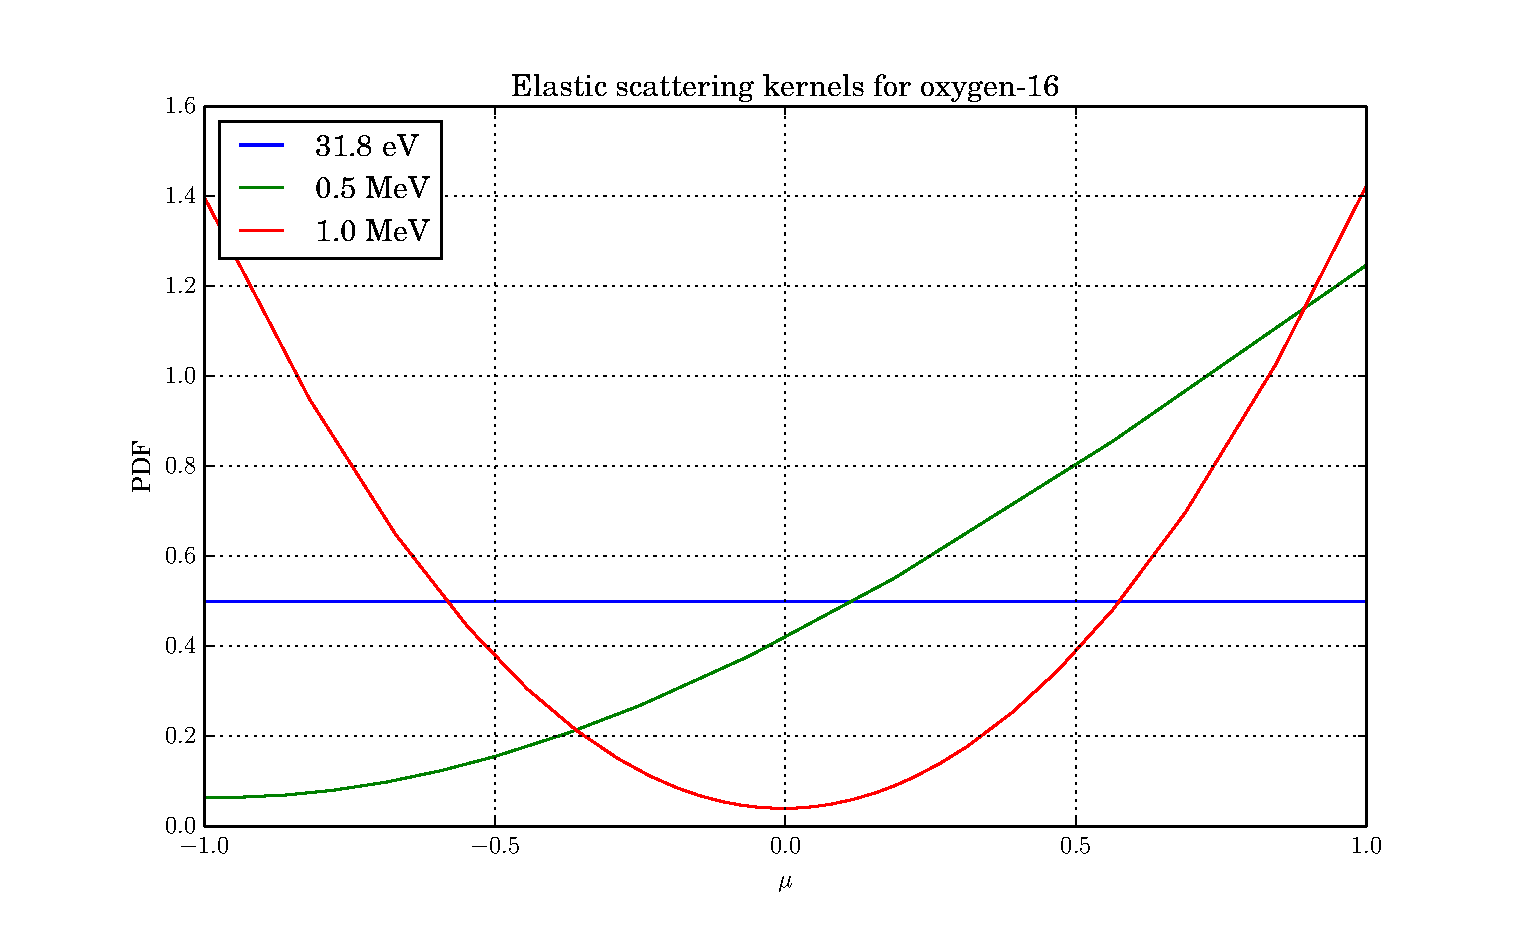
\includegraphics[width=0.8\textwidth]{graphics/scattering_anisotropy.eps}
     \caption{Elastic scattering anisotropy at high energies in oxygen-16.  \label{scattering_anisotropy}}
\end{figure}

It is essential to model this phenomena accurately since the scattering angle factors heavily into the energy exchange between the particles.  Figure \ref{scattering_error} shows what can happen when elastic scattering is treated as isotropic for all energies.  The figure shows the normalized flux per lethargy in a one meter cube of water with a 2 MeV point source at its center.  The neutron flux spectra immediately under scattering resonances are too large due to neutrons not losing enough energy in scattering events.  The large backward scattering probability causes more energy to be lost on average than purely isotropic scattering.

\begin{figure}[h!] 
  \centering
    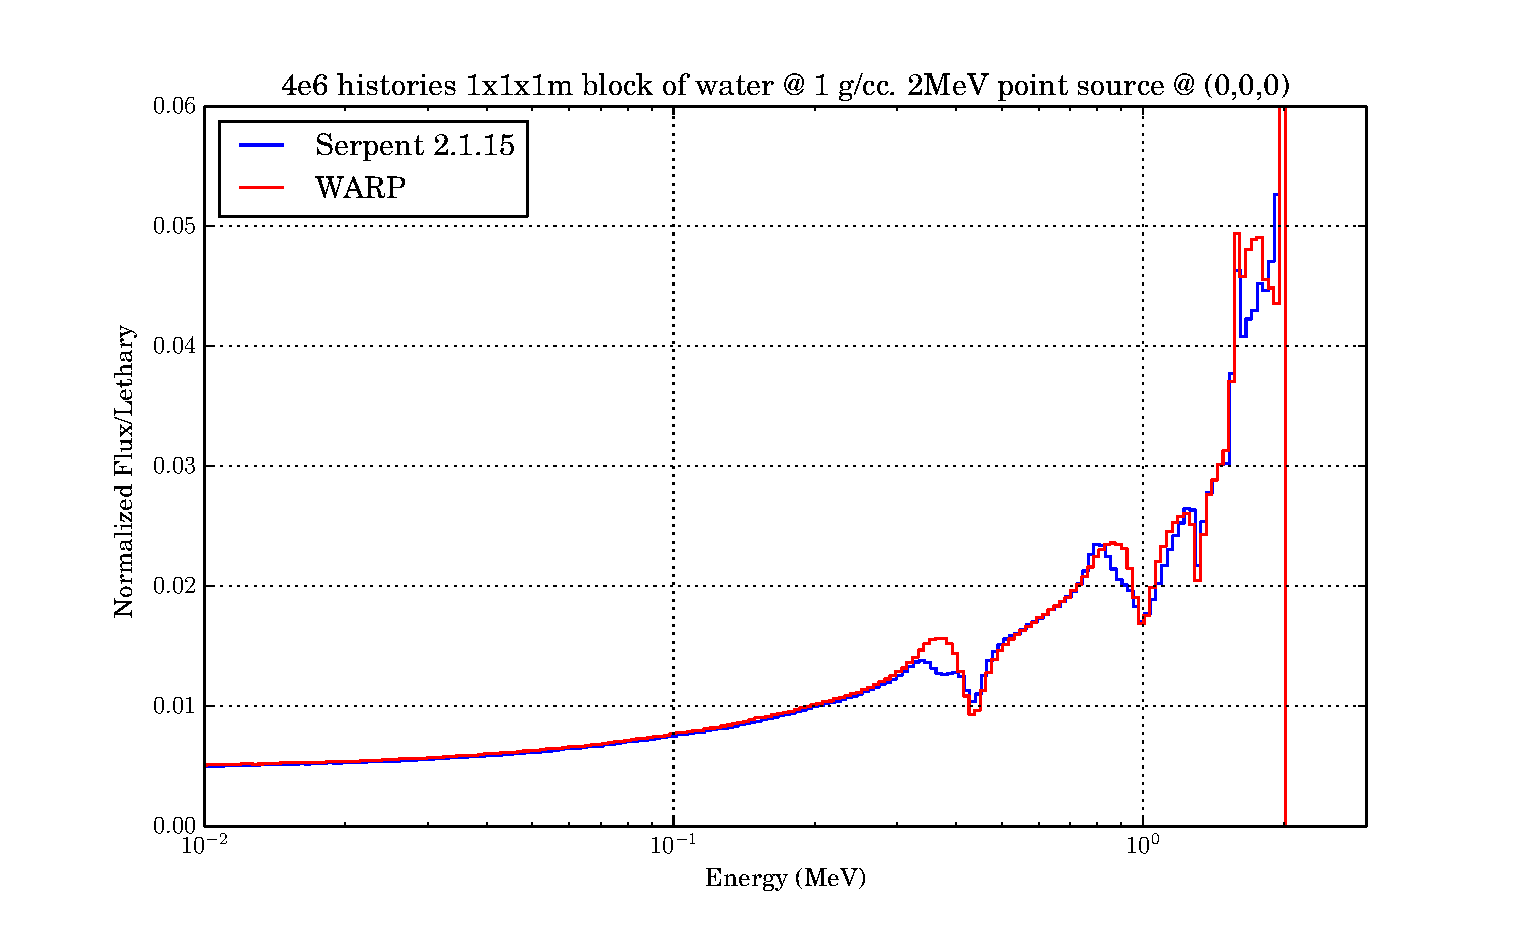
\includegraphics[width=0.8\textwidth]{graphics/scattering_error.eps}
     \caption{Error in the energy spectrum caused by treating elastic scattering as isotropic for all energies.\label{scattering_error}}
\end{figure}

After the target and neutron are transformed to the CM frame, the scattering CDF histogram interpolated and sampled as described in previous subsections.  Once the scattering angle is known, the rotated angle is calculated via Rodrigues' rotation formula shown in \eqref{RodriguesRot}.  The CM-rotated neutron velocity vector is then transformed back to the lab frame and the reaction is complete.

\subsubsection{Inelastic Reactions}

Inelastic level scattering is treated identically to elastic scattering except that the $Q$ value in \eqref{finalvCM} is now nonzero.  This value is reaction-specific and must be given by the data tables.  

Inelastic continuum scattering is treated differently, however.  Instead of having a well-defined kinematic formula relating the scattering angle to the final neutron energy, continuum reactions are defined by correlated scattering and energy tables.  They follow ENDF ``law'' number 44, the Kalbach-Mann correlated energy-angle scattering law \cite{mcnp} \cite{openmc}.  In this sampling scheme, a CDF is histogram or linearly-linearly interpolated and sampled from just like other reactions, except the sampled value is now a set of ``precompound factors,'' $R$, and ``angular slopes,'' $A$, instead of $\mu$ directly.  These values correspond to a secondary PDF, shown in \eqref{law44}, which is again sampled from to find $\mu$.

\begin{equation}
\label{law44}
PDF = \frac{A}{2 \sinh (A)} ( \cosh(A\mu)+R \sinh (A\mu))
\end{equation}

The sampling scheme for this probability distribution shown in \eqref{law44samp}, where $\xi_1$ and $\xi_2$ are two additional random numbers .  Since this is a correlated angle-energy distribution, there there is an energy value along with the factors $A$ and $R$ that corresponds to a CDF bin.  This sampled energy value is scaled via \eqref{energy_scaling} just like those from a tabular energy distribution, which is the topic of the next subsection \cite{3rdsampler}\cite{openmc}.

\begin{equation}
\label{law44samp}
\begin{split}
\mathrm{if} \: \xi_1 > R:  \quad T&=(2\xi_2-1)\sinh(A)\\
\mu &= \frac{\ln(T+\sqrt{T^2+1})}{A}\\
\mathrm{else: }  \qquad & \\
\mu &= \frac{ \ln(\xi_2 \exp(A) + (1-\xi_2)\exp(-A))}{A}
\end{split}
\end{equation}

\subsubsection{Tabular Energy Distributions}

Continuous, independent energy distributions, like those specified for fission spectra, have multiple CDFs specified at various incoming neutron energies.  Stochastic mixing probability $f$, shown in \eqref{mixing_prob}, is used to select if the lower-bounding or upper-bounding distribution will be sampled from for $E_i < E < E_{i+1}$.  After the distribution is selected, the CDF is sampled with histogram or linear-linear interpolation, which ever is specified in the library.  Once the sampled energy, $E_\mathrm{sampled}$, is calculated, it must be scaled to the bounding incoming energy bins to preserve any thresholds.  This is done via \eqref{energy_scaling} where $E_{i,\mathrm{first}}$ and $E_{i,\mathrm{last}}$ are the first and last energy values of the CDF in $E_i$; and $E_{i+1,\mathrm{first}}$ and $E_{i+1,\mathrm{last}}$ are the first and last energy values of the CDF in $E_{i+1}$ \cite{mcnp}.

\begin{equation}
\label{energy_scaling}
\begin{split}
E_a &= E_{i,\mathrm{first}} +  f( E_{i+1,\mathrm{first}} - E_{i,\mathrm{first}} ) \\
E_b &= E_{i,\mathrm{last}} +  f( E_{i+1,\mathrm{last}} - E_{i,\mathrm{last}} ) \\
\mathrm{if\:i+1\:sampled:} \quad \mathrm{diff} &= E_{i+1,\mathrm{last}}  - E_{i+1,\mathrm{first}}  \qquad E_\mathrm{start}= E_{i+1,\mathrm{first}}  \\
\mathrm{else:}          \qquad \quad       \mathrm{diff} &= E_{i,\mathrm{last}}  - E_{i,\mathrm{first}}  \qquad \qquad E_\mathrm{start}= E_{i,\mathrm{first}}  \\
E^\prime &=  E1  +  ( E_\mathrm{sampled} - E_\mathrm{start})  \frac{ E_b - E_a}{ \mathrm{diff} }  
\end{split}
\end{equation}


\subsection{Tallies}




\cite{jaakko}



\subsection{Neutron Sources}

So far, all that has been mentioned is how to handle the different reactions in a Monte Carlo neutron transport simulation.  This is important since reactions describe what happens to neutrons and where they go during their random walk, but how to handle \emph{where} they come from still needs to be defined.  The source terms on the right hand side of the neutron transport equation, other than the scattering source, have not been defined yet.  In this subsection, the other two source terms, the external source and the criticality source, are discussed.

\subsubsection{External Source}

An external, or fixed, source is simply a source which does not depend on the neutron population itself.  Physically, such a source could be from natural radioactive decay, an accelerator source, etc.  The only concern with an external source in a Monte Carlo simulation is in accurately measuring the response of the system, more specifically, the response of the system if it contains fissile material.  If a single neutron is ``shot'' into a multiplying material, all the secondary particles the primary neutron induces also need to be simulated in order to simulate the response of the system.  The number of secondary neutrons produced is fully defined by the multiplication factor since it gives the ratio of subsequent neutron generations.  An expression for the converge infinite series is shown in \eqref{sub_crit_mult}\cite{duderstadt}\cite{jaakko}.

\begin{equation}
\label{sub_crit_mult}
N_\mathrm{total} = N_0 + k N_0 + k^2 N_0 + \dots = N_0 \sum_{i=0}^\infty k^i = \frac{N_0}{1-k}
\end{equation}

This series only converges for $k<1$, which sets a restriction for fixed-source simulations.  If the multiplication factor is greater than one, it will require infinitely many secondary neutrons to be tracked, so this situation must be avoided.

\subsubsection{Fission Source, $k$-Eigenvalue Method}

When a fission source is specified, the simulation will run in a manner different to an external source problem.  The neutron source now depends on the neutron population itself, and a method must be used which directly ties the source to the population.  This is done by using any points where neutrons any secondary-producing reactions as source points for subsequent neutron histories.  When neutrons are born from these induced points, they of course must follow the emissions laws specified by the data.  For fission reactions, there is usually a tabulated energy spectrum, which is sampled and interpolated in the data-specified ways, and then scaled to the incoming energy bins via \eqref{energy_scaling}.  The angle is isotropic in the lab frame, and this is easily sampled via \eqref{iso_samp}.

\begin{equation}
\label{iso_samp}
\begin{split}
\phi &= 2 \pi \xi_1 \\
\mu= \cos \theta &= 2 \xi_2 -1
\end{split}
\end{equation}

In criticality simulations, the parameter of interest is usually the effective multiplication factor, $k_\mathrm{eff}$.  It is defined by \eqref{k_eff_batch}, where $N_{s,n}$ is the number of source neutrons in the current generation, and $N_{s,n+1}$ is the number of neutrons in the next generation \cite{jaakko}.  Calculating this quantity in a Monte Carlo simulation is straightforward, but generation information must be preserved.  Correct results cannot be obtained if yields from source particles in different generation are used to calculate the number of sources in the next generation.  This is why criticality source simulations are usually run in a batched mode where a preset number of source particles from a single generation are all transported until termination.  The secondary-producing reaction points are then used as the starting points for the next generation.  The generations are not interleaved, and correct values for the multiplication factor can be calculated.

\begin{equation}
\label{k_eff_batch}
k_{\mathrm{eff},n} = \frac{N_{s,n+1}}{N_{s,n}}
\end{equation}

Modeling the fission chain reaction is simple in Monte Carlo simulations when a system is exactly critical.  In batched criticality mode, the next generation of neutrons have starting points which are determined by the previous generation.  When the system is exactly critical, there is a one-to-one mapping of induced secondary neutrons to preset number of source particles to be transported in the next batch.  But when the system is sub- or super-critical, there is no longer a one-to-one mapping and starting points either have to be reused or discarded, respectively.  This is done by using the \emph{k-eigenvalue method}, which used by the Serpent code \cite{jaakko}.  After $k_\mathrm{eff}$ is calculated via \eqref{k_eff_batch}, it is used to renormalized the fission source of the next generation, i.e. the secondary yield values are divided by $k_\mathrm{eff}$.  This is an analog to dividing the fission source term in \eqref{time_ind_NTE} by $k_\mathrm{eff}$ to enforce the time derivative to be zero.  By dividing the yield values by $k_\mathrm{eff}$, the multiplication factor should be 1, and a one-to-one mapping is recovered.  

Since $k_\mathrm{eff}$ are continuous, calculating an integer value of secondary particles is done stochastically to preserve the aggregate mean.  The renormalized yield, $y_r$, is stochastically rounded based on a random number $\xi$ as shown in  \eqref{stoch_rounding}.  Doing this ensures that over a large batch size, the multiplication factor is renormalized as close to one as possible.  In the case where $y_r$ is slightly less than one, the last few source points from the previous generation are simply reused.  This should not introduce much bias in the results if the source distribution is converged.

\begin{equation}
\label{stoch_rounding}
\begin{split}
&y_r = \frac{\mathrm{yield}}{k_\mathrm{eff}} \\
\mathrm{if}\quad &y_r - \mathrm{floor}(y_r)<\xi \\
\mathrm{then:}\quad &y_r=\mathrm{ceil}(y_r) \\
\mathrm{else:}\quad &y_r=\mathrm{floor}(y_r)
\end{split}
\end{equation}

To start the simulation, a guess must be made for the initial points neutrons are born.  in some codes, one can specify a single initial point where all of the first generation neutrons are born.  As the simulation progresses, the source expands and converges to the true distribution.  The initial batches, or cycles, when the source distribution is far from the correct distribution are therefore discarded.  No quantities are accumulated and the multiplication factors values are not used in calculating the final value.  The discarded cycles only serve to converge the fission source so the accumulated quantities later in the simulation are not biased due to an incorrect source distribution.  In order to accelerated this process, WARP uses a similar method to Serpent to guess the initial source distribution.  The materials in the geometry are all flagged as fissile or non-fissile.  Then and uniform, random distribution of source neutrons are distributed across the geometry.  If the particles lies in a fissile material, it is recorded in a buffer.  This process is repeated until the required amount of source points are accumulated in the starting point buffer.  This method is called the \emph{flat source approximation}, and should require fewer cycles to be discard than the point source method since the initial distribution has spatial extent and fewer cycles will be needed to simply push neutrons into all geometrical regions \cite{jaakko}.

When all the cycles are complete, the individual estimates of $k_\mathrm{eff}$ are averaged to make a final estimate for the system.  This is typically called the \emph{generation estimate} of $k_\mathrm{eff}$ \cite{jaakko}.  As the simulation runs, a recursion relation can be made so the values for every cycle does not need to be stored individually.  Expressions for the generation estimate are shown in \eqref{k_eff_final}.  It may be of interest to keep values for every cycle in order to perform statistical checks to assure convergence, however.

\begin{equation}
\label{k_eff_final}
\begin{split}
\bar{k}_{\mathrm{eff},n} &= \frac{1}{n} \sum_{i=1}^{n} k_{\mathrm{eff},i} \\
\bar{k}_{\mathrm{eff},n} &= \frac{1}{n} \left[ k_{\mathrm{eff},n} + (n-1) \bar{k}_{\mathrm{eff},n-1}  \right]
\end{split}
\end{equation}


%%%%%%%%%%%%%%%%%%%%%%%%%%%%%%

\section{GPUs}

Now that the simulation methods have been framed,

Part of the reason GPUs are able to perform efficiently is do to their reliance on single instruction, multiple data (SIMD) execution.  This execution method uses the same instructions carried out over multiple pieces of data at the same time.  This reduces the amount of power used in control and therefore more math can be done per watt [citation definitely needed].  The GPU programming model abstracts SIMD execution by using threads, which can be thought of in the traditional sense . There are some tradeoffs, however, including limited on-board memory (currently 12 GB), limited cache and control space, and requiring data parallelism for full utilization.

Since all threads in a GPU thread block must execute the same instructions, having conditional statements based on random numbers can cause threads to be serialized, leading to resource under-utilization.  For example, in particle transport where a particle history is assigned to each thread, thread divergence mainly arises through particles undergoing different reactions based on the results of cross-section sampling.  Also, GPUs have even higher global memory latency than CPUs, up to 800 clock cycles on older cards, compared to about 50 cycles on a typical CPU.  It is also important to remember than GPUs are clocked much slower than CPUs, so the memory latency performance issue is even greater [5, 7]. 

Conventional CPU-based parallel Monte Carlo algorithms typically use the approach of one particle history per CPU thread.  Data is accessed when needed and threads execute completely independently of each other.  This is a task-parallel approach, the typical algorithm for which is shown in Figure 1, and works well on CPUs due to their large cache and control sizes (relative to cores) and the lower latency of accessing global memory (smaller penalty for random access).  This approach has been historically called history-based parallelism as well.  To fully utilize the computational power of GPUs, this approach must be modified.  Threads need to execute identical instructions and therefore must be in the same stage of the transport algorithm.  Studies have been done trying to directly port task-parallel Monte Carlo algorithms to GPUs with some success, most notably that of Liu, et. al. [10], and they suggest that a data-parallel approach similar to those used in vector computers should be employed [1, 10].  This approach is also called event-based parallelism since events, such as scattering or surface crossing, are done in parallel for many particles at once.

Figure 2 shows the data parallel algorithm used to maintain thread coherence (i.e. executing the same instructions) between GPU threads.  It is similar to the vectorized approach used with the early vector computers, which also were able to use a single-instruction, multiple-data (SIMD) execution model [1, 2].  A single-instruction multiple-thread (SIMT) and SIMD are similar in the sense that identical instructions are carried out across different pieces of data, but SIMT allows threads to act independently, albeit with a performance penalty.   The two main features of Figure 2 are that independent GPU kernel launches are used for each step of the transport chain and that the kernels operate on a large set of particle data (as opposed to transporting one particle at a time).  By doing this, the transport cycle is broken into steps in which a single task, such as determining reaction type or finding boundary intersection, is performed across large dataset of particles and threads can be kept more coherent.

another brief introduction.  

advantages

pitfalls, weaknesses

\subsection{Supercomputing}

how and why they came to be used for supercomputing.

\subsection{Architecture}

SIMD, threads

\subsection{Memory}

speed, levels, etc.  limitations 

\subsection{CUDA}

kernels

\subsection{OptiX}

optix stuff

%%%%%%%%%%%%%%%%%%%%%%%%%%%%%%

\section{Previous Works}

talk about the work that other people did

\section{Preliminary Studies}

all my prelim work to motivate this project

\subsection{2D Scattering Game}

\begin{figure}[h!] 
  \centering
    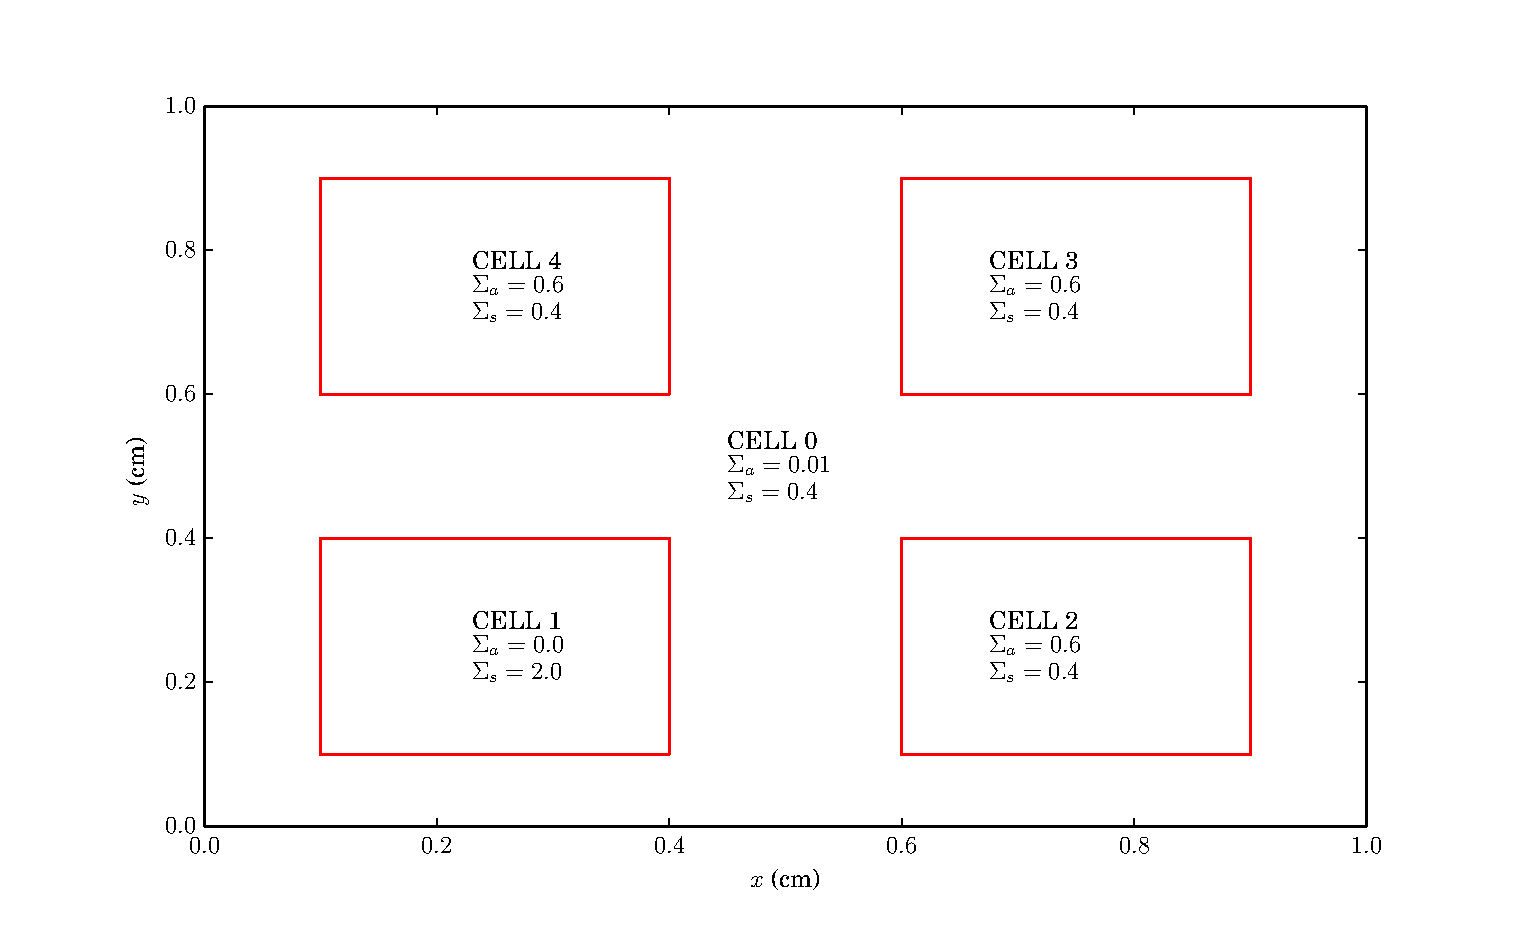
\includegraphics[width=0.8\textwidth]{graphics/prelim_geom.eps}
     \caption{The 2D geometry of the scattering test.  \label{prelim_geom}}
\end{figure}


\subsection{Ray Tracing with OptiX}
\label{sec:prelim}

%%%%%%%%%%%%%%%%%%%%%%%%%%%%%%

\section{Scope in Detail}


